\chapter{Fair loss function from noise robustness}\label{chap:ftl}

In this chapter we propose a novel loss function inspired by label noise robustness methods to fair classification problems. The core of this proposal consists in using transition matrices as parameters to a proper loss correction~\cite{Patrini2017}, with matrices values as factors to redistribute unbalanced bias across different groups within the sensitive feature.

\section{Preliminaries}

The presence of noise in data can substantially decrease model performance in classification problems. Noise can be defined as non systematic errors that obscures the relationship between features of an instance and its class~\citep{Frenay2014,Hickey1996,Quinlan1986}. Two types of noise are found in literature, in features (or attributes) and in labels (or classes). Feature noise affects observed values, e.g. by adding a small Gaussian noise on each feature during measurement. Likewise, label noise change the observed label assigned to an instance, e.g. by randomly inverting labels in a binary classification problem. Although feature noise could affect model performance, label noise is potentially more harmful, since we frequently have many features and only one label. Note that in label noise only the observed label of an instance is affected, its true class remains the same.

The label noise taxonomy considers three types of noise: Noisy Completely at Random, Noisy at Random, and Noisy Not at Random~\citep{Frenay2014}. Figure~\ref{fig:taxonomia} presents the statistical dependency between features $X$, class $Y$, observed label $\tilde{Y}$ and the occurrence of error E, i.e. $E=1$ when $Y \neq \tilde{Y}$. The simplest type is Noisy Completely at Random, where the occurrence of error $E$ not depend on $X$ and $Y$, e.g. randomly flipping labels on a binary classification problem. In Noisy at Random, the occurrence of error $E$ depends only on $Y$, e.g. randomly flipping labels on binary classification with different rates for positives and negatives classes. Noisy Not at Random considers the occurrence of error $E$ depending on both $Y$ and $X$, e.g. flipping labels on binary classification with different rates for each group of instances of a certain feature.


 \begin{figure}[!htb]
 \centering
\caption{Noise taxonomy from a statistical perspective. (a) completely random noise (NCAR), (b) random noise (NAR) and (c) non-random noise (NNAR). The arrows correspond to the statistical dependencies. For clarity, the dependency between $X$ and $Y$ was placed as a dashed arrow.}
 \label{fig:taxonomia}
 \scalebox{1.0}{%
    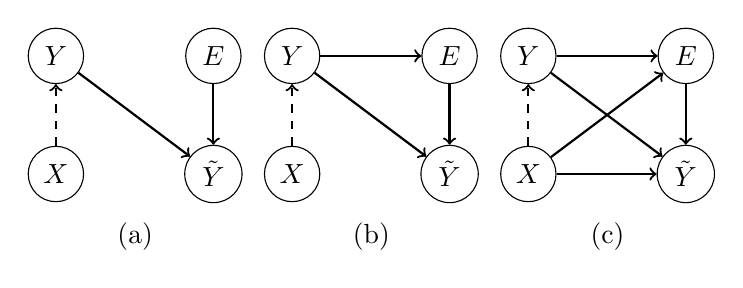
\begin{tikzpicture}[main_node/.style={circle,draw,minimum size=2em,inner sep=3pt]}]

     \node[main_node] (1) at (-1, 0) {$Y$};
     \node[main_node] (2) at (-1, -1.5)  {$X$};
     \node[main_node] (3) at (1, -1.5) {$\tilde{Y}$};
     \node[main_node] (4) at (1, 0) {$E$};
     \path[->,draw,thick]
     (1) edge node {} (3)
     (4) edge node {} (3)
     ;

     \path[->,dashed,thick]
     (2) edge node {} (1)
     ;

     \node[below=2cm] at (current bounding box.base) {(a)};

     \begin{scope}[xshift=3cm,grow=right,baseline]

     \node[main_node] (1) at (-1, 0) {$Y$};
     \node[main_node] (2) at (-1, -1.5)  {$X$};
     \node[main_node] (3) at (1, -1.5) {$\tilde{Y}$};
     \node[main_node] (4) at (1, 0) {$E$};

     \path[->,draw,thick]
     (1) edge node {} (3)
     (4) edge node {} (3)
     (1) edge node {} (4)
     ;

     \path[->,dashed,thick]
     (2) edge node {} (1)
     ;

     \node[below=2cm,xshift=1.5cm] at (current bounding box.base) {(b)};

     \end{scope}

     \begin{scope}[xshift=6cm,grow=right,baseline]
     \node[main_node] (1) at (-1, 0) {$Y$};
     \node[main_node] (2) at (-1, -1.5)  {$X$};
     \node[main_node] (3) at (1, -1.5) {$\tilde{Y}$};
     \node[main_node] (4) at (1, 0) {$E$};

     \path[->, draw,thick]
     (1) edge node {} (3)
     (4) edge node {} (3)
     (1) edge node {} (4)
     (2) edge node {} (3)
     (2) edge node {} (4)
     ;

     \path[->,dashed,thick]
     (2) edge node {} (1)
     ;

     \node[below=2cm,xshift=3cm] at (current bounding box.base) {(c)};

     \end{scope}
 \end{tikzpicture}
 }
 \end{figure}

Many label noise robustness methods can be found on literature, in this work we highlight the \textit{backward} and \textit{forward} loss corrections, proposed by \cite{Patrini2017} using concepts of loss factorization~\citep{Patrini2016}. Those loss correction techniques considers a NAR label noise, which is described by a transition matrix $T$ such as
\begin{equation}
    T_{i,j} = P(\tilde{Y} = y_j|Y = y_i),
\end{equation}
where $\mathcal{Y} = \{y_1, y_2, \ldots, y_c\}$ is the set of all possible class labels. Transition matrix includes corruption probabilities for every possible label combination, each value represents the probability of one label be corrupted onto another. This matrix is row-stochastic and not necessarily symmetric across the classes.
\begin{equation} \label{eq:backward}
    \ell^{\leftarrow}(P(\tilde{Y}|X)) = T^{-1} \ell(P(\tilde{Y}|X))
\end{equation}

The backward loss correction is defined by Equation~\ref{eq:backward} to an arbitrary loss function $\ell$ and a transition matrix $T$. The backward loss correction involves a linear combination of the loss values for each observed label, using coefficients that depends on the probability that each observed label reflects the true class. Intuitively, we are reweighting the loss according to the noise probabilities of each label using the inverse of T and thus somehow going one step back, reverting the noise effects. This corrected loss is unbiased and can be minimized with any conventional back-propagation algorithm, making it flexible to include within different training techniques and data pipelines.
\begin{equation} \label{eq:forward}
    \ell^{\rightarrow}(P(\tilde{Y}|X)) = \ell(T^{\top} P(\tilde{Y}|X))
\end{equation}

However, backward correction requires matrix inversion, which may not exist or may lead to numerical instabilities if the transition matrix T is ill-conditioned. Although there is possible solutions to a bad condition number of T, one should consider using the forward correction, a backward variation proposed by \cite{Patrini2017} to avoid this issue, as defined in Equation~\ref{eq:forward}. While backward acts on the loss itself, forward corrects model predictions. Forward correction does not have the same theoretical guarantees as backward, but offers a label noise robustness, ensuring that the learned model is the minimize over the clean distribution without the need of matrix inversion.

Now we discuss classification methodologies that operate in the presence of label noise. While our research does not directly tackle fairness problems in the presence of label noise, we highlight relevant works that, akin to ours, bridge the domains of fairness and noise in machine learning research.

Some recent works deal with fairness problems in the presence of noise. For example, the sensitive attribute available could be noisy, which could distort the effects of fairness intervention. In this context, \cite{Lamy2019} uses noise-rate estimators from the label noise literature to change a fairness model. Also, \cite{Fogliato2020} proposes a framework for assessing how assumptions on the noise across groups affect the predictive bias properties in risk assessment models. Furthermore, \cite{Wang2020} considers the consequences of naively relying on noisy protected group labels while proposing two new optimization approaches with sensitive attribute noise robustness. A denoised version of the selection problem to deal with noisy sensitive attributes is proposed in \cite{Mehrotra2021}. Lastly, \cite{Celis2021} proposes an optimization framework for classification in the presence of noisy protected attributes.

There is also the perspective of dealing with the proxy features divergence or covariance. A theoretical approach to this issue identifying potential sources of errors can be found in \cite{Prost2021}. The problem of measuring group fairness in ranking based on divergence with proxy features is investigated by \cite{Ghazimatin2022}. A framework of fair semi-supervised learning in the pre-processing phase can be found in \cite{Zhang2022}, which includes predicting labels for unlabeled data, a resampling method, and ensemble learning to improve accuracy and decrease discrimination.

Another research direction is considering how fair models perform in the presence of NNAR label noise, where error rates of corruption depend both on the label class and the membership of a protected subgroup. In this scenario \cite{Wang2021} addresses the problem of fair classification and \cite{Wu2022} provides a general framework for rewriting the classification risk and the fairness metric in terms of noisy data and thereby building robust classifiers. In \cite{Ghosh2023} a study about the presence of noise in the protected attribute can be found.

Furthermore, many recent works deals with fairness under semi-supervised settings considering censored data, that is, for some individuals the class label is not available due censorship~\cite{WZhang2022,WZhang2023_a,WZhang2023_b,WZhang2023_c}. In this scenario, the main approach is to use some technique to estimate the missing data instead of removing the instance from training data. This is closely related to the previous problems of fair learning under noisy data. In censored fairness problems noise can be interpreted as a kind of censorship, as the original data affected by noise is not available.

Bias and noise are two related phenomena, both corrupt data affecting models trained with this data. For example, if noise disproportionately affects different groups this potentially produces unfairness in models that uses this data in training~\citep{Wang2021}. For example, we could have positive true class ($Y = 1$) flipped into negative labels ($\tilde{Y} =0$) more frequently in the protected group ($A = 1$) than in privileged group ($A = 0$). Simultaneously, the negative class ($Y = 0$) could be more frequently flipped into positives observed labels ($\tilde{Y} = 1$) within privileged/unprotected group ($A = 0$). This scenario could lead to a undetected higher false negative rate to protected group and higher false positive rate to privileged group. In this case the Noisy Not at Random data would be a source of negative social bias.

As referred before, in \cite{Mehrabi2019} a non-exhaustive list of bias types was presented. In the scenario described above, the incorrect measurement of the true class resulted in a different observed label ($Y \neq \tilde{Y}$), which could be classified as a \textit{Measurement Bias}. Similarly, a Noisy Not at Random data could lead to a \textit{Population Bias}, where the characteristics of the population represented in the data differ from those of the original target population.

It can be challenging to distinguish between label noise and bias in certain scenarios, specially when noise disproportionately affects different social groups. Although there is some overlapping, they are distinct phenomena. Label noise is a stochastic process that is considered independent and unintentional~\citep{Frenay2014}, whereas bias is rooted in historical and social issues and could be intentional. Furthermore, even noise-free data, correctly represented by observed features and labels, may be unfair since the social phenomena that produce this data could be biased against some groups.

Previous studies on fair machine learning have largely concentrated on understanding how noisy or censored data affects fair learning and on mitigating these effects. Thus, the objective of this work is not to theoretically deal with fair machine learning as a label noise problem or incorporate noisy classes or attributes in fairness problems. In contrast, our approach is inspired by label noise techniques, but with a distinct goal: not merely to analyze or mitigate the impact of noise or censorship, but to directly address and reduce unfairness itself.

To achieve a competitive trade-off between performance and fairness in the proposed method, we discuss multi-objective optimization within the context of fair machine learning. A model that substantially decreases model performance to reduce unfairness may not be a viable option, as low performance could harm all groups affected by the model's decisions, including protected groups. Similarly, a model projected to be a fair alternative that keeps performance almost intact, but with little or even no gain in fairness, is not practically relevant. It is possible that fine-tuning this trade-off could result in a fairer solution that achieves better performance than traditional methods, but this is not the case for most practical problems. Achieving this balance is one of the most challenging tasks in fair machine learning.

In this context, an interesting approach is to deal with fair machine learning as a Multi-Objective Optimization (MOO) problem, where predictive performance and fairness metric are the objectives, which could be defined according Equation~\ref{def:moo}, where $\lambda$ is a parameter configuration in the space $\Lambda$, $\rho: \Lambda \mapsto [0,1]$ is a model performance metric and $\varphi: \Lambda \mapsto [0,1]$ a fairness metric. The set of all optimal solutions is called Pareto front, where one objective cannot be improved without sacrificing another. In this setting there is no single $\lambda^*$ optimal solution, but a set of solutions forming a Pareto front~\citep{pareto1906manuale}.

\begin{align}\label{def:moo}
\max &\hspace{1ex} (\rho(\lambda), \varphi(\lambda)) \\
\text{subject to} &\hspace{1ex} \lambda\in\Lambda \nonumber
\end{align}

One of the most frequent approach to deal with MOO problems like these is to combine the multiple function outputs to a single scalar, which is called scalarization. Therefore, we could describe a general scalarization setup to Equation~\ref{def:moo} according Equation~\ref{def:scalarized_moo}. The effectiveness of this approach is that is also possible to use single objective optimization techniques to tackle the MOO optimization problem. In this scenario a relevant issue is to select a scalarization setup capable of promote a proper trade-off of all the objectives thorough the optimization process given the optimization method.

\begin{equation}\label{def:scalarized_moo}
\arg\max\limits_{\lambda\in\Lambda} G(\lambda) = (\rho(\lambda), \varphi(\lambda))
\end{equation}

The fairness-accuracy Pareto front is formally described in \cite{Wei2022}, which demonstrate that many existing fairness methods are performing a linear scalarization scheme and argues that it has several limitations in recovering Pareto optimal solutions. Instead, authors proposes a Chebyshev scalarization scheme, that is theoretically superior than linear scheme. A characterization of the accuracy-fairness trade-off as a Pareto front can be found in \cite{Liu2022}. Also, \cite{Mercier2018} proposes a stochastic multi-gradient based in original stochastic multi-gradient to Multi-Objective Optimization.

Another remarkable use of MOO in Fair Machine Learning is to perform a Fair Hyperparameter Optimization, which provides a model agnostic approach with flexibility to apply in multiple machine learning pipelines. A time-efficient Baysian Optimization approach can be found in \cite{Schmucker2020}, combining scalarization techniques with the bandit-inspired Hyperband \citep{Li2016} algorithm to Hyperparameter Optimization in context of fairness.

A general objective function to be used with some popular off-the-shelf hyperparameters optimization techniques combining model performance and fairness in a flexible setting can be found in \cite{Cruz2021}. The authors argues that in fairness context the Pareto front is most often convex, thus proposes a simple scalarizing function that could be applied to reduce $G$ to a single scalar with weighed $l_p$-norm. Also, they argue that \cite{GIAGKIOZIS2015338} demonstrate the the  use  of $l_p$-norms with a high $p$ value leads to slower convergence. Thus, the optimization metric $g(\lambda) = ||G(\lambda)||_1$ is optimized according Equation~\ref{eq:moo_smoothed_2}, where $\alpha$ is the relative importance of predictive performance and fairness and $\lambda$ is a parameter configuration in the space $\Lambda$. In experiments, $\alpha$ is fixed at $0.5$, giving same importance to both objectives.

\begin{equation} \label{eq:moo_smoothed_2}
    G(\lambda) = \alpha \cdot \rho(\lambda) + (1-\alpha) \cdot \varphi(\lambda)
\end{equation}

A Multi-objective SVMOptimizer with Dataset Constraints is proposed by \cite{Goh2016}, where the objective is to minimize multiple objectives on real-world datasets, such as misclassification error and positive prediction at specific rate to some population. A custom reinforcement learning algorithm directly modeling performance and fairness as objectives is proposed by \cite{Petrovic2021}. Authors proposes using as reward function the difference between model performance (Area Under the ROC Curve) and three different fairness metrics (Statistical Parity, Equal Opportunity and Equalized Odds), each one with its respective importance coefficient. In experimental setups only one of those coefficient are different from zero. Thus, the optimized metric could be written as $G(\lambda) = \rho(\lambda) - \alpha \cdot \varphi(\lambda)$, where $\alpha$ is the relative importance of fairness.

\section{Fair Transition Loss} \label{sec:proposal}

We propose a novel fair classification method inspired by techniques used for classification in the presence of label noise. By using some features of label noise methods that redistribute probabilities for unbalanced noise across classes, our approach re-weights prediction probabilities to reduce disparities in favorable and unfavorable outcomes across social groups. This proposal was originally inspired by \cite{Braida2018}, that applies label noise techniques in order to achieve label noise robust collaborative filtering,

Whereas forward loss correction~\citep{Patrini2017} uses a transition matrix with corruption probabilities for every label combination in the case of NAR, fair classification problems are more related to NNAR. While forward loss correction uses a transition matrix with corruption probabilities for each label combination, as in the case of NAR, fair classification problems align more with NNAR scenarios. In NNAR, the probability of corruption depends not only on the true class but also on features, analogous to how bias in fairness problems is directed against certain groups. Here our correction does not revert a random label corruption from the true class, but a potentially unfair prediction. While noise label techniques, like forward~\citep{Patrini2017}, aims to correct the prediction targeting a unknown true class using the available noisy label, analogously the proposed technique focus on correcting predictions chasing the unknown fair class using the available unfair label. Despite those are distinct phenomena, the corrections works the same way, adjusting the probabilities of predictions produced by a machine learning model during the training. 

Thus, our proposal is a prediction probability loss reweighting technique that accounts different rates to each group of the sensitive feature, instead of using the same correction to every individual. A correction method that incorporates different probabilities for protected and unprotected groups could be more effective in mitigating bias during the learning phase. Specifically, we want a forward-based correction that takes into account a different matrix to each group of sensitive features, not only one transition matrix as used in label noise techniques. In this scenario, each group of sensitive feature have its own correction, with its own rates for each class combination. Ideally, if we can find an appropriate transition matrix that describes the bias to each group in a specific problem, we can apply a correction that attenuates those negative effects by reweighting model's predictions in the learning process.

Next, we formally present Fair Transition Loss. For purpose of clarity we follow the same structure available at \citep{Patrini2017}, with the pertinent changes to our scope. The Fairness Transition Matrix $T_a$ is defined with some abuse of notation to the group $A=a$ of the sensitive feature as 
\begin{equation}
    T_{a,i,j} = P(\tilde{Y} = y_j|Y = y_i, A=a),
\end{equation}
where label space $\mathcal{Y} = \{y_1, y_2, \ldots, y_c\}$, $c$ the number of classes, $Y=y_i$ is the unknown fair class and $\tilde{Y}=y_j$ is the available and 
possibly unfair label. Here, $T_{a,i,j}$ is the probability of the fair class $Y=y_i$ being unfairly labeled as $\tilde{Y}=y_j$ to an individual of the group $A=a$ due negative social bias. Therefore, suppose that there is an inversible link function $\psi : \Delta^{c-1} \rightarrow \mathbb{R}^c$, where $\Delta^{c-1} \subset [0,1]^c$ is the $c$-simplex, the simplex in a $c$-dimensional space. Thus, a composite loss function, denoted by $\ell_{\psi} : \mathcal{Y} \times \mathbb{R}^c \rightarrow \mathbb{R}$ if it can be written as a decomposition of $\psi^{-1}$, that is,

\begin{equation}
    \ell_{\psi}(Y, h(X)) = \ell(Y, \psi^{-1}(h(X)), 
\end{equation}
where $h:\mathcal{X} \rightarrow \mathbb{R}^c$ is a standard artificial neural network with multiple layers using activation functions, and $h(X)$ is the output o this neural network to a given input $X$. For example, to cross entropy loss function the softmax is the inverse link function. Proper loss functions are those that can be directly used to estimate class probabilities. The minimizer of a proper composite loss has the particular form of the link function applied to the conditional class probabilities $P(Y|X)$. Adding a new conditioning to this formulation, to an individual from group $A=a$ we have

\begin{equation} \label{eq:argmin_ftl}
    \argmin\limits_{h}\mathbb{E}_{X,Y}\ell_{\psi}(Y, h(X|A=a)) = \psi(P(Y|X,A=a)).
\end{equation}

Fair Transition Loss consists in correcting model's predictions with the same technique as forward, but taking into account the sensitive attribute value when choosing the transition matrix. In Theorem~\ref{theorem:ftl} the Fair Transition Loss is formally defined, with a guarantee about its minimizers.

\begin{theorem}\label{theorem:ftl}
    Suppose that the Fairness Transition Matrix $T_a$ for a given sensitive attribute $A=a$ is non-singular. Given a proper composite loss $\ell_{\psi}$, define the Fair Transition Loss as
    \[\FTL_{\psi}(h(X|A=a)) = \ell(T^{\top}_a \psi^{-1}(h(X|A=a))).\]
    Then, the minimizer of the corrected loss under the unfair distribution is the same as the minimizer of the original loss under the fair distribution:
    \[  \argmin\limits_{h}\mathbb{E}_{X,\tilde{Y}}\FTL{\psi}(Y, h(X|A=a)) = \argmin\limits_{h}\mathbb{E}_{X,Y}\ell_{\psi}(Y, h(X|A=a)).\]
\end{theorem}
\begin{proof}
    First notice that:
    \begin{align} \label{eq:proof_ftl}
        \FTL_{\psi}(Y, h(X|A=a)) &= \ell(Y, T^{\top}_a \psi^{-1}(h(X|A=a))) \nonumber \\
        &= \ell_{\phi}(Y, h(X|A=a)),
    \end{align}
    where we denote $\phi^{-1} = \psi^{-1} \circ T_a^{\top}$. Equivalently, $\phi = (T_a^{-1})^{\top} \circ \psi$ is invertible by composition of invertible functions, its domain is $\Delta^{c-1}$ as of $\psi$ and its codomain is $\mathbb{R}^{c}$. The last loss in Equation~\ref{eq:proof_ftl} is proper composite with link $\phi$. Finally, from Equation~\ref{eq:argmin_ftl}, the loss minimizer over the unfair distribution is
    \begin{align}
        \argmin\limits_{h}\mathbb{E}_{X,\tilde{Y}}\ell_{\phi}(Y, h(X|A=a)) &= \phi(P(\tilde{Y}|X,A=a)) \\
        &= \psi((T_a^{-1})^{\top}) P(\tilde{Y}|X,A=a) \\
        &= \psi(P(Y|X,A=a)),
    \end{align}
    that proves the Theorem by Equation~\ref{eq:argmin_ftl} once again.
\end{proof}

Considering a common scenario with only two groups in sensitive attributes (protected and privileged), we can correct the model's predictions using two different fair transition matrices. One with rates applied while learning instances from the protected group, and the other with rates applied while learning instances from the privileged group. Formally, to the sensitive feature $A \in \{0,1\}$, let $T_0$ the transition matrix associated with privileged/unprotected group ($A = 0$) and $T_1$ with the protected group ($A = 1$), $\FTL$ can be computed as

\begin{equation}
    \FTL(P(\tilde{Y}|X)) = (1-A) \cdot \ell(T^{\top}_0 P(\tilde{Y}|X)) + A \cdot \ell(T^{\top}_1 P(\tilde{Y}|X)),
\end{equation}
which in a standard batch learning, consists in alternating the transition matrix applied according instance's sensitive attribute.

Furthermore, to a common binary classification problem, where there is a positive (favorable) class and a negative (unfavorable) class, and two groups from sensitive feature (protected and privileged), we have two $2\times2$ transition matrices. Intuitively we are choosing rates to increase or decrease the probability of each group to be classified with the positive or negative prediction. We name those rates associated with increasing the probability to achieve the positive outcome as \textit{promotion} rate, and those associated with increasing the probability to receive the negative outcome as \textit{demotion} rate. As the transition matrix is row-stochastic, we can describe $T_0$ and $T_1$ as
\begin{equation} \label{eq:transition_matrices}
    T_0 = \left[\begin{array}{cc}
        1-d_0 & d_0\\
        p_0 & 1-p_0\\
    \end{array}\right],\;
    T_1 = \left[\begin{array}{cc}
        1-d_1 & d_1\\
        p_1 & 1-p_1\\
    \end{array}\right],
\end{equation}
where $d_0$ is the privileged demotion rate, $p_0$ the privileged promotion rate, the $d_1$ protected demotion rate, and $p_1$ the protected promotion rate. With an appropriate combination of $d_0$, $p_0$, $d_1$, $p_1$ we can define a transition matrix pair that should be able to reweight model's predictions with $FTL$ to achieve fairer results with a reasonable model performance. The central problem in our methodology thus relies in choosing these rates, which can be seen as an hyperparameter optimization problem.

Our hyperparameter optimization problem consists in finding an optimal trade-off between fairness and performance, which can be described as a MOO problem, as defined in Equation~\ref{def:moo}. Here, the hyperparameter configuration is $\lambda = (d_0, p_0, d_1, p_1)$. Since the transition matrix is row stochastic these parameters are sufficient to define $T_0$ and $T_1$. We want to maximize model performance $\rho(\lambda)$ and minimize fairness metric $\varphi(\lambda)$. 

\begin{equation} \label{eq:obj_fn}
    G(\lambda) = \rho(\lambda) - \varphi(\lambda).
\end{equation}

Following some MOO approaches to fair machine learning, we will use a linear scalarization setup to define the optimization metric~\citep{Schmucker2020,Petrovic2021}. As we yet have four hyperparameter to fine-tune, and in \cite{Cruz2021} the relative importance $\alpha$ is fixed at $0.5$, we choose a simple and intuitive objective function in Equation~\ref{eq:obj_fn} to maximize without the parameter $\alpha$, i.e., giving same importance to fairness and performance. In Equation~\ref{eq:obj_fn} we establish a simple objective to optimize, but one might need to consider a different formulation depending on the specific problem at hand.


\section{Experimental setup} \label{sec:experimental}

In this section, we detail the experimental setup employed to benchmark our model against relevant in-processing fair classification models found in standard fairness toolkits, namely, Prejudice Remover~\citep{Kamishima2012}, Adversarial Debiasing~\citep{Zhang2018}, and Gerry Fair Classifier~\citep{kearns18a}. We use the implementation of these methods from AI Fairness 360 toolkit~\citep{aif360-oct-2018}. The baseline is a Standard MLP using two hidden layers with $100$ hidden units each, $ReLU$ activation function, batch size of $64$, $50$ epochs early stopped at $3$ epochs without improvement~\citep{Li2020} and softmax in output, trained with ADAM optimizer~\citep{KingmaB14} with learning rate at $3\mathrm{e}{-4}$. The only difference between baseline MLP and Fair Transition Loss MLP is that baseline uses standard Binary Cross Entropy Loss. The Gerry Fair Classifier implementation uses the False Negative Rate as its fairness definition and in Adversarial Debiasing classifier the hidden size is $100$ units. Additionally, we compare the Fair Transition Loss within the Adaptive Priority Reweighting~\cite{HuXT23}, a promising fairness promoting technique focused on improving generalization, which outperformed many recent methods such as \cite{jiang2020identifying}, \cite{mroueh2021fair}, and \cite{roh2020fairbatch}.

Our methodology consists of two phases: hyperparameter tuning and testing. In the hyperparameter tuning phase we perform a Bandit-Based pruning approach using HyperBand~\citep{Li2018} with Tree-structured Parzen Estimator Sampler (TPE)~\citep{bergstra2011} over 100 trials. Those techniques achieves better solutions to multi-objective hyperparameter optimization in the same number of trials than conventional approaches like Grid Search and Random Search~\citep{Morales-Hernandez2023}. At each trial fitness function is evaluated by performing a complete training and validation, where both model performance and fairness metrics are assessed. The fitness function is computed based on the objective defined in Equation~\ref{eq:obj_fn}. This same experimental procedure can be adapted to utilize other hyperparameter tuning algorithms such as FairRandom Search, Fair TPE, and Fairband~\citep{Cruz2021}.

Once the best hyperparameters are selected, we proceed to the testing phase, where a new training is conducted using those optimal hyperparameters. After this training, we evaluate the model's performance on a separate test set that was not used during the hyperparameter tuning phase, which are reported. This complete tuning-training-testing described is repeated $15$ times with dataset re-sampling then we proceed to comparison. Here the re-sampling consists in shuffling the whole dataset before splitting, which is better described further in this section.

As the objective defined in Equation~\ref{eq:obj_fn} can be achieved with different performance and fairness metrics, we compare the proposed method with other relevant in-processing techniques from literature in different optimization scenarios. In addition to Accuracy (Acc.) as performance metric, we also evaluate the Mathews Correlation Coefficient (MCC), which has advantages over F1 score and Accuracy in binary classification evaluation~\citep{chicco2020advantages}. To this performance metric, $1$ means a perfect prediction according true class, $-1$ a complete inversion and $0$ an average random outcome. As fairness metric we consider Statistical Parity (Stat. Parity, Definition~\ref{def:demo_parity}), Equal Opportunity (Eq. Opp., Definition~\ref{def:eq_opp}) and Equalized Odds (Eq. Odds, Definition~\ref{def:eq_odds}). Thus we have the following optimization scenarios: MCC and Statistical Parity; MCC and Equal Opportunity; MCC and Equalized Odds; Accuracy and Statistical Parity; Accuracy and Equal Opportunity; Accuracy and Equalized Odds.

\begin{table}[ht]
\centering
\caption{Hyperparameters search ranges or options of each method.}\label{tab:hyperparameters}
{\footnotesize
\begin{tabular}{lll}
\toprule
Method & Parameter & Range/options \\ \midrule
 Standard MLP (baseline) & dropout & $[0.0,\,0.2]$  \vspace{1ex} \\
 Prejudice Remover~\citep{Kamishima2012} & $\eta$ & $[0.0,\,50.0]$ \vspace{1ex} \\
 Adversarial Debasing~\citep{Zhang2018}& $\alpha$ & $[0.0,\,1.0]$  \vspace{1ex} \\
 Gerry Fair Classifier~\citep{kearns18a} & $C$ & $[0.0,\,20.0]$ \\
 &  $\gamma$ & $\{0.1,\,0.01,\,0.001\}$ \vspace{1ex} \\
 Adaptive Priority Reweighting~~\citep{HuXT23} & $\alpha$ & $[0.0,\,10000.0]$ \\
 &  $\eta$ & $[0.5, 3.0]$ \vspace{1ex} \\
 Fair Transition Loss & $d_0,p_0,d_1,p_1$ & $[0.0,\,1.0]$ \\
 &  dropout & $[0.0,\,0.2]$ \\
\bottomrule
\end{tabular}
}
\end{table}

Table~\ref{tab:hyperparameters} presents the methods hyperparameters along with their corresponding search ranges or options. While each method may possess a varying number of hyperparameters and range sizes, all are optimized under the same conditions and number of configurations to guarantee a balanced comparison. In Figure~\ref{fig:fitness_sensibility} we present a brief sensibility analysis on the fitness functions with different fairness and performance values over those six optimization scenarios listed before. Here we perform a complete hyperparameter tuning with HyperBand and TPE over $100$ trials using the baseline model (Standard MLP) with the Adult Income dataset optimizing the hyperparamers reported on Table~\ref{tab:hyperparameters}. This sensibility analysis aims better present the linear objective function behavior within performance and fairness metrics evaluated in this study.

\begin{figure}[!ht]
\centering
\caption{Sensibility analysis on optimized fitness functions within different performance and fairness metrics. Results from complete hyperparameter tuning through $100$ trials with baseline model over the Adult Income dataset.}
    \label{fig:fitness_sensibility}
    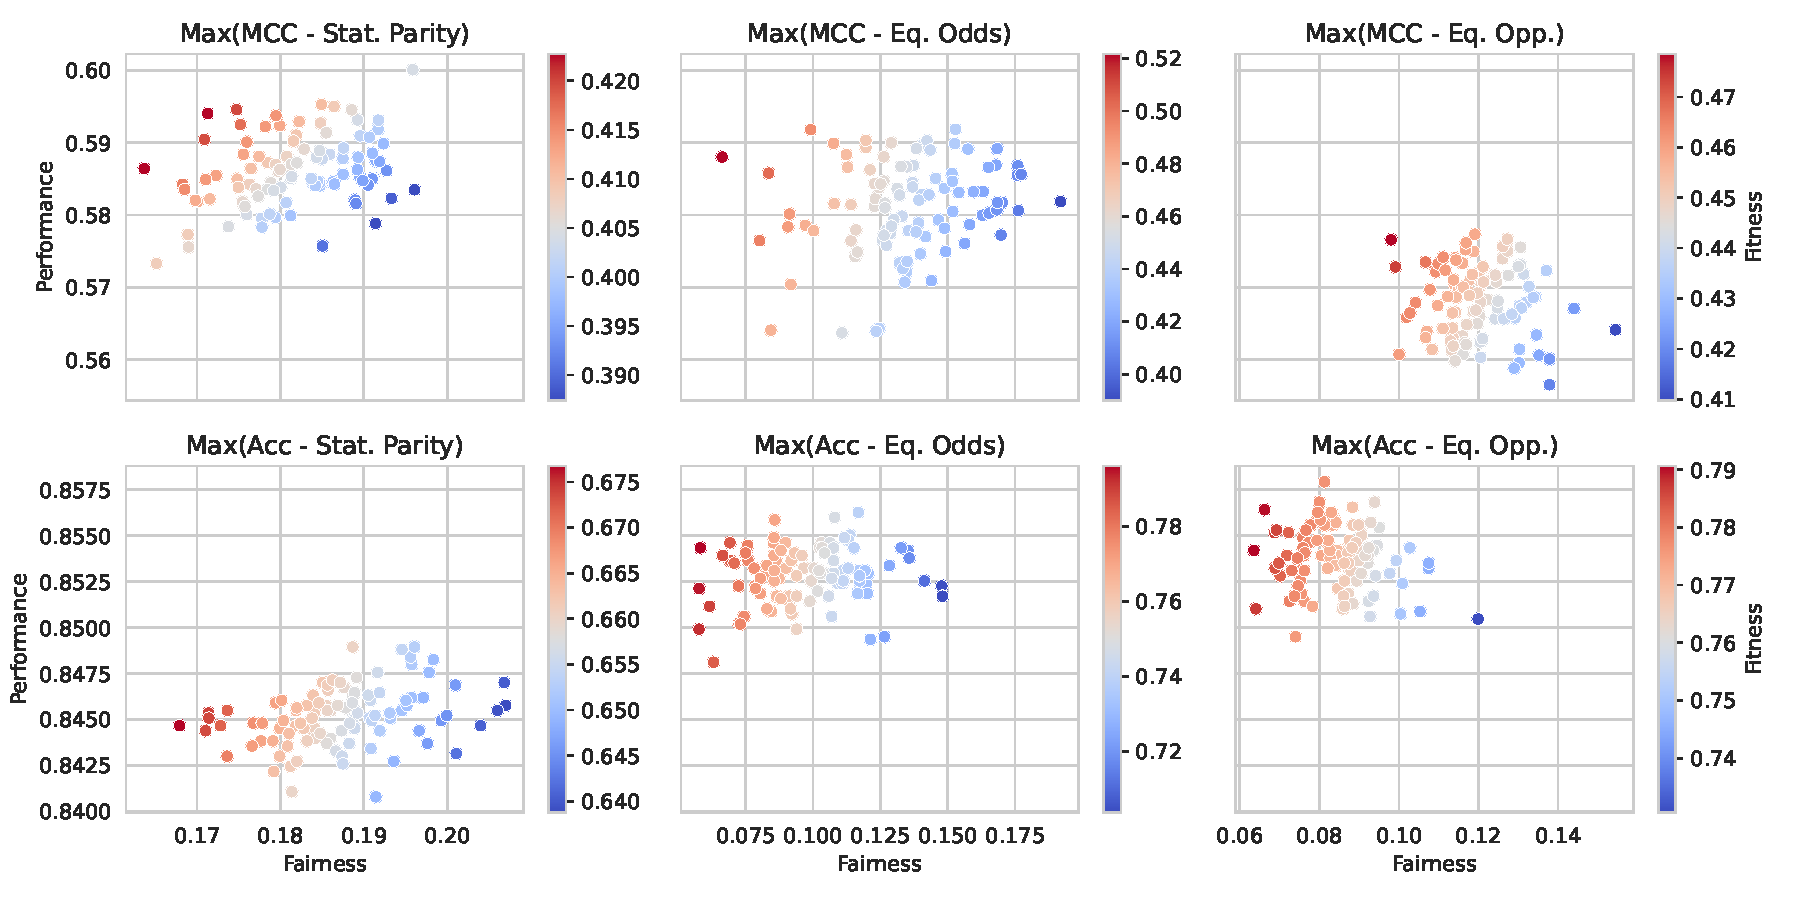
\includegraphics[width=1\linewidth]{images/fitness_sensibility.pdf}
\end{figure}

Each plot in Figure~\ref{fig:fitness_sensibility} illustrates the fitness value corresponding to specific performance and fairness metrics. The color scheme in the plots represents the fitness values, with higher values in red and lower values in blue. On the $x$-axis, we have the fairness metric, where a lower value is preferable. The $y$-axis represents the performance metric, with higher values being preferred. The color gradient in these plots demonstrates the linear relationship between fitness and variations in the corresponding performance and fairness metrics. It is important to note that the scale of the fairness metric is significantly smaller than that of the performance metric. However, it is sufficiently to act as a penalization. The general fitness function in the scenarios described is capable of producing results with reduced bias while maintaining similar performance levels. Although each metric combination has different scales, each hyperparameter tuning experiment uses only one metric combination at a time, ensuring consistency in the optimization process.

On these plots we used the fitness and performance levels obtained through the TPE sampler with HyperBand pruning during the hyperparameter tuning phase using the baseline model, as previously described. In this setting, the solution (i.e., the combination of hyperparameters) that yields the best fitness value is selected for a new complete training phase. This involves assessing metrics on test data not used in the previous phase. To ensure robust evaluation, the dataset is reshuffled, re-split into train, validation and test segments, and this entire process is repeated over 15 iterations.

To properly compare this set of $15$ results of each method, we conduct an Almost Stochastic Order (ASO) test \citep{dror2019deep}, which is a significance test suitable for comparing complex machine learning models with various hyperparameters. The ASO test involves evaluating a set of metrics through multiple samplings of a Collection of Statistics (in this case assessed in test phase using random resampling) to compare one method against another. The $ASO(A, B)$ function yields a value in the range $[0, 1]$, given two methods $A$ and $B$. If $ASO(A, B)$ is lesser than $0.5$, we can reject the null hypothesis and conclude that method $A$ outperforms method $B$ in the given task. That is, method $A$ produces stochastically larger values than method $B$ for a given metric. The lower the $ASO(A, B)$ value, the stronger the evidence that $A$ is superior to $B$ in that particular task, which can be interpreted as a confidence interval. Therefore, we perform pairwise comparisons between all methods for each optimization scenario outlined previously and for each dataset.

%\subsection{Datasets description}\label{sec:datasets}

Our experiments uses common datasets used in Fair Classification problems, namely \textit{Adult Income}~\citep{misc_adult_2}, \textit{German Credit}~\citep{misc_statlog_(german_credit_data)_144}, \textit{Bank Marketing}~\citep{misc_bank_marketing_222}, and \textit{COMPAS Recidivism}~\citep{misc_compas}. We use the dataset readers available in the AI Fairness 360 toolkit~\citep{aif360-oct-2018} with its standard configurations. Instances with missing data are removed.

\begin{table}[ht]
    \centering
    \caption{Dataset details used in this work, including performance and fairness metrics assessed to a standard classifier without tuning, and the maximum correlation between sensitive feature and the other features.}\label{tab:datasets}
    {\footnotesize
    \begin{tabular}{lrrrr}
        \toprule
        \multirow{2}{*}{\shortstack[l]{Dataset}} & \multirow{2}{*}{\footnotesize\shortstack[l]{Adult\\ Income}} & \multirow{2}{*}{\footnotesize\shortstack[l]{Bank\\ Marketing}} & \multirow{2}{*}{\footnotesize\shortstack[l]{COMPAS\\ Recidivsm}} & \multirow{2}{*}{\footnotesize\shortstack[l]{German\\ Credit}} \\ \\
        \midrule
\# Features & 102 & 57 & 401 & 58 \\
\# Instances & 45222 & 30488 & 6167 & 1000 \\
Sensitive Attribute & sex & age & race & sex \\
Positives & 24.78\% & 12.66\% & 54.45\% & 70.00\% \\
Negatives & 75.22\% & 87.34\% & 45.55\% & 30.00\% \\
Privileged & 67.50\% & 97.17\% & 34.05\% & 69.00\% \\
Unprivileged & 32.50\% & 2.83\% & 65.95\% & 31.00\% \\
Accuracy & 0.846 & 0.906 & 0.358 & 0.685 \\
MCC & 0.572 & 0.553 & -0.275 & 0.000 \\
Stat. Parity. & 0.192 & 0.106 & 0.172 & 0.074 \\
Equal Opportunity & 0.094 & 0.145 & 0.120 & 0.043 \\
Equalized Odds & 0.092 & 0.094 & 0.163 & 0.122 \\
Maximum Correlation & 0.527 & 0.364 & 0.826 & 0.593 \\
        \bottomrule
    \end{tabular}
    }
\end{table}


Table~\ref{tab:datasets} present dataset details used in this work, including the number of features before pre-processing, the count of valid instances, the proportion of positive and negative labels, the sensitive feature considered in experiments, the proportion of privileged and unprivileged groups within the corresponding sensitive feature, reference performance and fairness metrics using a standard Random Forest Classifier with $1000$ classifiers without tuning, and the maximum correlation coefficient between the sensitive feature and the other features. The maximum correlation is useful to assess whether it is possible to use another feature as proxy to the sensitive feature, which is commonly referred as redlining effect~\citep{Pedreschi2008}.

The \textit{Adult Income} dataset presents a classification task to predict whether an individual earns more than $50,000$ per year. This dataset consists of $48,842$ instances sourced from the U.S. 1994 Census database. The sensitive attribute used in this task is sex, with the male group considered privileged and the female group protected (unprivileged). In the \textit{German Credit} dataset, the task consists of classifying $1,000$ individuals described by a set of attributes as good or bad credit risks. Similar to the \textit{Adult Income} dataset, here we use sex as the sensitive attribute, with the male group considered privileged and the female group protected. The \textit{Bank Marketing} classification task aims to predict whether $45,211$ clients will subscribe to a term deposit after direct marketing campaigns (phone calls) by a Portuguese banking institution. In this case, the sensitive feature is age, where individuals under the age of $25$ are considered unprivileged, while those aged $25$ and older are considered privileged. The \textit{COMPAS} dataset presents around $80,000$ criminal records from the Broward County Clerk’s Office. The task here is to predict whether a defendant will recidivate in the next two years. The sensitive feature in this case is race, with Caucasians as the privileged group and non-Caucasians (Black and Hispanic) as unprivileged.

For all datasets, the data preparation process is the same, one-hot encoding for categorical features and standardize the numerical features. We perform a random split, with $80\%$ allocated for the hyperparameter tuning phase and the remaining $20\%$ reserved for evaluating metrics in the test phase. Within the hyperparameter tuning phase, this corresponding fraction of data is further randomly split, with $80\%$ assigned to training and $20\%$ to validation. The validation set allows us to assess metrics and compute the fitness function for each hyperparameter configuration. In datasets where there is originally some kind of split (e.g., train set and test set in separate files), all available data is merged and then shuffled to produce new splits at each run.

\section{Results and discussion} \label{sec:results}

This section summarizes our results, comparing Fair Transition Loss (FTL) with the baseline Standard MLP (MLP) and some relevant fair in-processing methods: Adversarial Debiasing (AD), Prejudice Remover (PR), Gerry Fair Classifier (GFC) and Adaptive Priority Reweighting (APW).

\begin{table}[ht]
    \centering
    \caption{Almost Stochastic Order test comparing Fair Transition Loss fitness. Values under $0.5$ (in bold) mean that FTL outperforms corresponding method in such optimization scenario.} \label{tab:aso_compare}
    {\footnotesize
    \begin{tabular}{llccccc}
    \toprule
     \multirow{2}{*}{\shortstack[l]{Fairness/Performance\\Metric}} & Dataset & MLP & AD & PR & GFC & APW \\ \\
\midrule
\multirow{4}{*}{\shortstack[l]{Statistical Parity\\MCC}} & Adult Income & \textbf{0.00} & \textbf{0.15} & 1.00 & \textbf{0.00} & 1.00 \\
 & Bank Marketing & \textbf{0.01} & \textbf{0.00} & \textbf{0.00} & \textbf{0.00} & \textbf{0.00} \\
 & Compas Recidivism & \textbf{0.01} & \textbf{0.25} & \textbf{0.00} & \textbf{0.02} & \textbf{0.00} \\
 & German Credit & \textbf{0.28} & \textbf{0.30} & \textbf{0.39} & \textbf{0.21} & \textbf{0.28} \vspace{1ex}\\

\multirow{4}{*}{\shortstack[l]{Equal Opportunity\\MCC}}  & Adult Income & \textbf{0.01} & \textbf{0.00} & \textbf{0.05} & \textbf{0.00} & 0.93 \\
 & Bank Marketing & 0.81 & \textbf{0.18} & \textbf{0.24} & \textbf{0.09} & 0.77 \\
 & Compas Recidivism & \textbf{0.00} & 1.00 & \textbf{0.00} & 0.66 & 1.00 \\
 & German Credit & 1.00 & \textbf{0.23} & 0.84 & 0.78 & 0.76 \vspace{1ex}\\

\multirow{4}{*}{\shortstack[l]{Equalized Odds\\MCC}}  & Adult Income & \textbf{0.03} & \textbf{0.28} & \textbf{0.42} & \textbf{0.00} & \textbf{0.00} \\
 & Bank Marketing & \textbf{0.46} & \textbf{0.18} & \textbf{0.12} & \textbf{0.02} & \textbf{0.18} \\
 & Compas Recidivism & \textbf{0.01} & 0.58 & \textbf{0.00} & \textbf{0.07} & \textbf{0.00} \\
 & German Credit & 1.00 & \textbf{0.07} & 1.00 & \textbf{0.31} & 1.00 \\
\midrule
\multirow{4}{*}{\shortstack[l]{Statistical Parity\\Accuracy}}  & Adult Income & \textbf{0.01} & \textbf{0.26} & \textbf{0.32} & \textbf{0.00} & 0.53 \\
 & Bank Marketing & \textbf{0.25} & 1.00 & 1.00 & 0.76 & 0.82 \\
 & Compas Recidivism & \textbf{0.00} & 1.00 & \textbf{0.10} & 1.00 & \textbf{0.00} \\
 & German Credit & 1.00 & \textbf{0.26} & 1.00 & 1.00 & 1.00 \vspace{1ex}\\

\multirow{4}{*}{\shortstack[l]{Equal Opportunity\\Accuracy}} & Adult Income & 0.89 & 0.97 & 1.00 & \textbf{0.23} & 0.98 \\
 & Bank Marketing & 1.00 & \textbf{0.39} & 0.81 & 1.00 & 1.00 \\
 & Compas Recidivism & \textbf{0.01} & 0.78 & \textbf{0.00} & \textbf{0.10} & 1.00 \\
 & German Credit & 1.00 & 0.64 & 1.00 & 1.00 & 1.00 \vspace{1ex}\\

\multirow{4}{*}{\shortstack[l]{Equalized Odds\\Accuracy}} & Adult Income & \textbf{0.01} & \textbf{0.21} & \textbf{0.19} & \textbf{0.00} & 1.00 \\
 & Bank Marketing & 0.76 & \textbf{0.40} & 0.82 & 1.00 & 1.00 \\
 & Compas Recidivism & \textbf{0.01} & \textbf{0.45} & \textbf{0.00} & \textbf{0.01} & \textbf{0.00} \\
 & German Credit & 1.00 & \textbf{0.12} & 1.00 & 1.00 & 1.00 \\

\bottomrule
\end{tabular}


    }
\end{table}

As we have multiple optimization scenarios with different objective functions and datasets, and to each of them multiple runs, we present in Table~\ref{tab:aso_compare} the results of the ASO test described before, which allow us to properly compare each method to FTL. Values under $0.5$ (in bold) mean that we can reject the null hypothesis, i.e., FTL produces stochastically larger fitness than method in respective column for a objective and dataset. Lower values indicate stronger evidence. The complete results with mean and standard deviation of fitness, performance and fairness can be found in tables~\ref{tab:complete_mcc_parity} to ~\ref{tab:complete_acc_odds} to a fairness-performance trade-off analysis.

In $69$ of $120$ comparison scenarios from Almost Stochastic Order test (Table~\ref{tab:aso_compare}), it is possible to claim that FTL outperforms its competitor, i.e., FTL produces stochastically higher fitness values. Despite these positive results, one can argue that the proposed technique only adds extra hyperparameters that increase models flexibility to achieve higher fitness values. In other words, are we effectively describing bias in datasets by transition matrices as claimed before? To address this, we showcase various FTL hyperparameter combinations selected during the tuning phase described in Section~\ref{sec:experimental}, comparing with corresponding dataset information available at Table~\ref{tab:datasets}. We perform this analysis using \textit{Adult Income} dataset. The corresponding hyperparameters can be found in Table~\ref{tab:found_hyperparameters}. Here, high values mean that FTL alters the corresponding probabilities, while values close to zero indicate minimal interference by the method.

\begin{table}[ht]
    \centering
    \caption{Fair Transition Loss hyperparameters chosen by optimizing different metrics in \textit{Adult Income} dataset.} \label{tab:found_hyperparameters}
    {\footnotesize
    \begin{tabular}{lcccc}
        \toprule
        \multirow{2}{*}{\shortstack[l]{Objective}} & \multirow{2}{*}{\footnotesize\shortstack[c]{$d_0$\\Priv. Dem.}} & \multirow{2}{*}{\footnotesize\shortstack[c]{$p_0$\\Priv. Prom.}} & \multirow{1}{*}{\footnotesize\shortstack[c]{$d_1$\\Prot. Dem.}} & \multirow{2}{*}{\footnotesize\shortstack[c]{$p_1$\\Prot. Prom.}} \\ \\
        \midrule
        MCC and Stat. Parity & $0.056$ & $0.076$ & $0.043$ & $0.878$ \\
        MCC and Eq. Opp. & $0.292$ & $0.455$ & $0.329$ & $0.575$ \\
        MCC and Eq. Odds & $0.037$ & $0.165$ & $0.005$ & $0.432$ \\
        Acc. and Stat. Parity & $0.470$ & $0.110$ & $0.023$ & $0.446$ \\
        Acc. and Eq. Opp. & $0.389$ & $0.326$ & $0.311$ & $0.530$ \\
        Acc. and Eq. Odds & $0.497$ & $0.286$ & $0.228$ & $0.094$ \\
        \bottomrule
    \end{tabular}}
\end{table}


When optimizing for MCC and Statistical Parity, there's a notable high value for protected promotion. This value is compatible with the high corresponding fairness metric for this dataset, approximately $0.19$ without correction. This increases the likelihood that an unprivileged instance receives a favorable outcome. Since statistical parity only compare the probability of a positive outcome across groups (ignoring true class) this is enough. The other hyperparameters presents low values. In contrast to the previous case, optimizing Equal Opportunity requires compatible false negative rates. Optimizing this fairness metric within MCC produces the effect of promoting both privileged and protected, although protected with higher values. This produces the effect of reducing false negatives at all, since the method enhances the probability of a positive outcome. This effect is counterbalanced with intermediate demotion rates to both groups through a finetuning to keep MCC. Note that Equal Opportunity values without correction to this dataset is not as high as Statistical Parity. To optimize Equalized Odds within MCC it is necessary to keep both false negatives and false positives comparable across groups, which lead to a less intense intervention when compared to Equal Opportunity. Here remains the high values to protected promotion to achieve fairness.

There is a remarkable difference between hyperparameters found through optimizing Accuracy and MCC. While MCC handles unbalanced classes effectively, Accuracy only measures the probability of correctly predicting an instance. If the dataset is unbalanced it is possible to achieve high Accuracy only by predicting the label of the more frequent class. In this dataset, only about a quarter of the instances are positives, which can lead to more frequent negative outcomes to achieve higher Accuracy. Results optimizing for Accuracy show significantly higher demotion rates compared to those from MCC optimization, both to privileged and protected groups. From this analysis, it's evident that the proposed methodology effectively describes and mitigates bias in a dataset according to a given fairness definition and while keeping targeted performance metric at a reasonable level.

Now we discuss the results to each objective, starting with MCC and Statistical Parity. To this objective Fair Transition Loss consistently outperforms all methods at all classification tasks, except Prejudice Remover (PR) and Adaptive Priority Reweighting (APW) in \textit{Adult Income}. Figure~\ref{fig:boxplot_mcc_parity} presents a box-plot comparison, where we can see that FTL, PR and APW are effectively drawn. While FTL and APW has little bit higher values, PR presents smaller variance. AS PR is a regularized logistic regression, it is a smaller model than FTL, which can explain the also smaller variance.

\begin{figure}[!ht]
\centering
\caption{Fitness values optimizing MCC and multiple fairness metrics.}
\begin{subfigure}{.32\linewidth}
    \caption{Statistical Parity}
    \label{fig:boxplot_mcc_parity}
    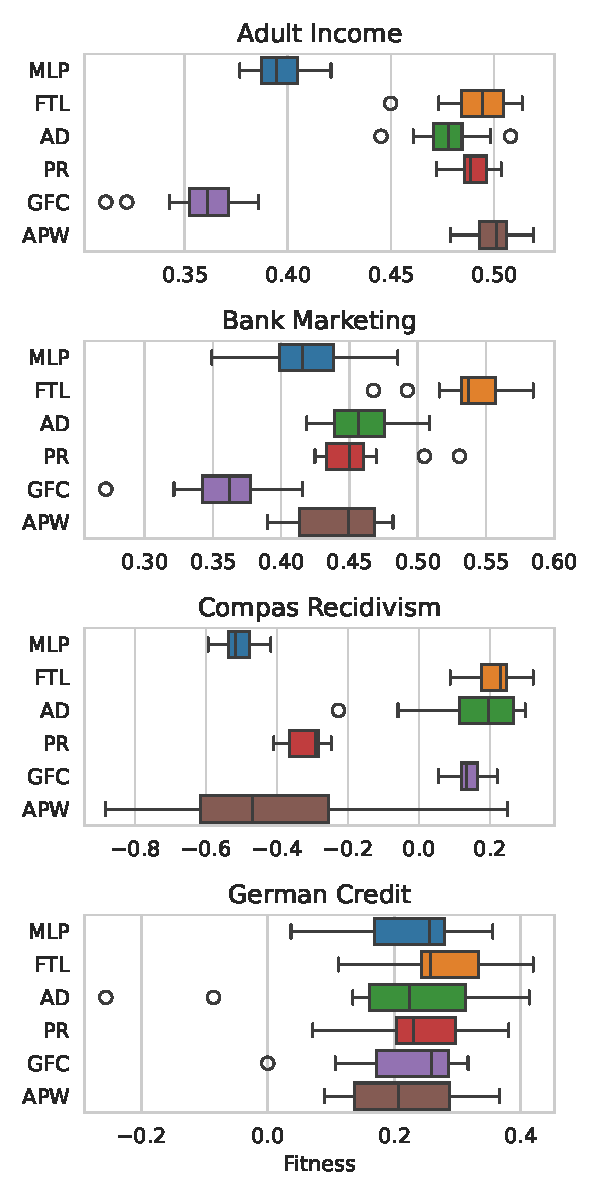
\includegraphics[width=1\linewidth]{images/boxplot_mcc_parity.pdf}
\end{subfigure}
\begin{subfigure}{.32\linewidth}
    \caption{Equal Opportunity}
    \label{fig:boxplot_mcc_opp}
    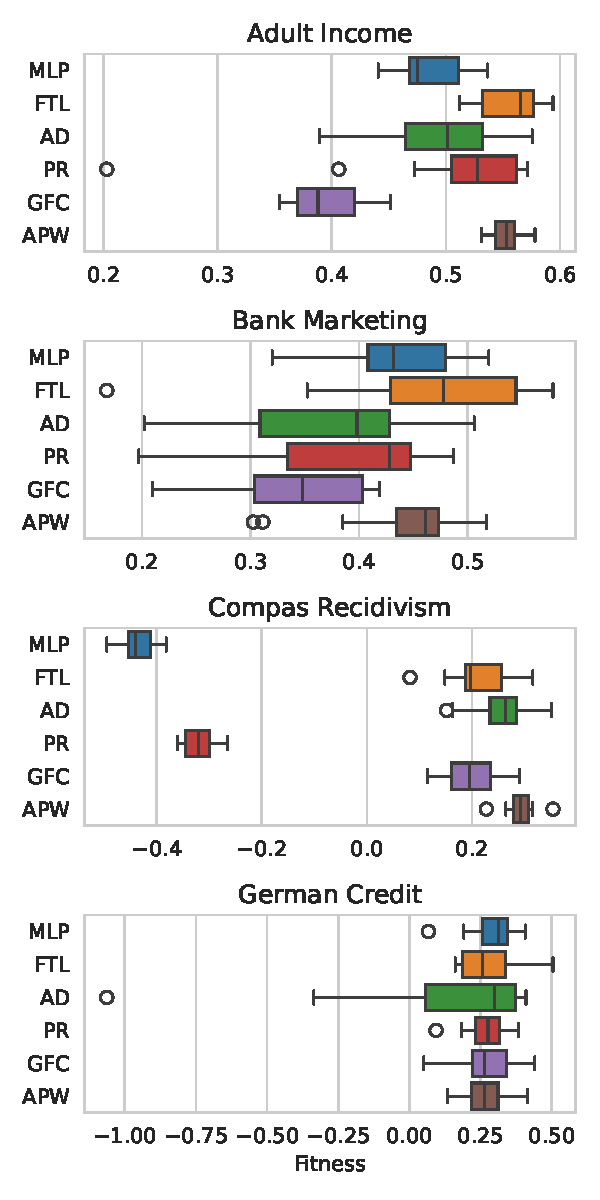
\includegraphics[width=1\linewidth]{images/boxplot_mcc_opportunity.pdf}
\end{subfigure}
\begin{subfigure}{.32\linewidth}
    \caption{Equalized Odds}
    \label{fig:boxplot_mcc_odds}
    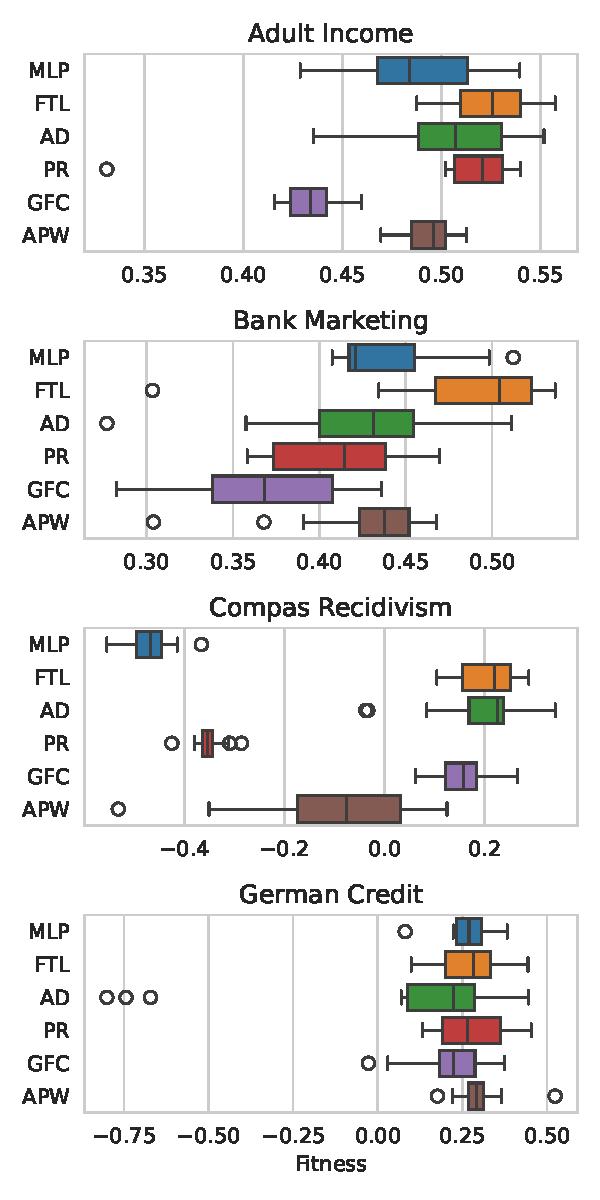
\includegraphics[width=1\linewidth]{images/boxplot_mcc_odds.pdf}
\end{subfigure}
\end{figure}

When comparing the optimization results for MCC and Equal Opportunity, FTL consistently outperforms its counterparts in most scenarios. Here we have only one discrepancy, as APW presents slightly advantage over FTL on \text{COMPAS} dataset. Also, on German Credit dataset all methods achieved similar results. Given the small size of this dataset, we theorize that all methods, barring AD, have reached the Pareto front — meaning, any further improvements in fairness would necessitate a proportional sacrifice in performance. This equilibrium between baseline (MLP), FTL, PR, GFC and APW is evident in Figure~\ref{fig:boxplot_mcc_opp}.

The sub-optimal results of AD can likely be attributed to the dataset's limited size; with merely $1000$ instances, this dataset might be too small for the an adversarial model like AD train effectively. This pattern of AD underperforming persists across subsequent classification tasks involving this dataset. Interestingly, also with the exception of AD, we notice that the variance in results for most optimization scenarios is smaller than in other classification tasks. This observation further underscores our Pareto front hypothesis and suggests that the classification task's simplicity may contribute to the reduced variability in outcomes.

When optimizing for MCC and Equalized Odds, we find that the results are consistent, with FTL outperforming its counterparts in most scenarios. Notably, within the \textit{German Credit} dataset, FTL surpasses not just AD but also GFC. Since GFC primarily relies on the False Negative Rate for its fairness definition, it has a natural advantage when optimizing for Equal Opportunity compared to Equalized Odds, which requires maintaining equitable False Positive and False Negative Rates. As observed in the previous comparisons, Figure~\ref{fig:boxplot_mcc_odds} underscores that the baseline, FTL, PR and APW seem to hit the Pareto front for this dataset.

Upon examining FTL's results when optimizing for MCC across all the fairness metrics evaluated, it's evident that FTL consistently  superior results compared to its counterparts. Specifically, FTL achieves stochastically higher fitness values in $44$ out of the $60$ scenarios evaluated. Given the inherent challenges associated with optimizing MCC compared to Accuracy, we attribute FTL's dominance in the MCC optimization to its capability of effectively capturing the bias idiosyncrasies of the dataset and the specified performance and fairness metrics trough transition matrices.

Furthermore, it's noteworthy that both the baseline and PR models substantially underperform across all optimization scenarios in the \textit{COMPAS Recidivism} classification task. This dataset, characterized by its complexity with $401$ features, might be at the heart of these subpar results. We theorize that the this lack of performance could be due to an insufficiently large model to navigate such a high-dimensional space, especially when we observe, as indicated in Table~\ref{tab:datasets}, that the standard performance on this dataset is relatively low.

When turning our attention to results obtained by optimizing Accuracy, we must first reiterate its inherent simplicity as a performance metric compared to MCC. Given its nature, it allows models to attain high values simply by predicting the label of the predominant class. In such circumstances, it is comparatively easier to reach the Pareto front. Even under these conditions, FTL displays commendable competitiveness. Although it achieves stochastically higher fitness values in $25$ of the $60$ scenarios, this rate is notably less than what we observed when optimizing for MCC. By juxtaposing Figures~\ref{fig:boxplot_acc_parity},~\ref{fig:boxplot_acc_opp},~and~\ref{fig:boxplot_acc_odds} with Table~\ref{tab:aso_compare}, we discern that in scenarios where FTL does not have the upper hand, it still competes closely with its counterparts. This very close results are primarily attributed to multiple methods simultaneously approaching the Pareto front. Likely when optimizing for MCC using Equal Opportunity as fairness metric, APW presents slightly advantage over FTL on \text{COMPAS} dataset.

A particularly straightforward fair classification task emerges when optimizing for Accuracy and Statistical Parity within the \emph{Adult Income} dataset. With this pronounced class imbalance, models can lean into over-predicting the majority class, thereby aligning the probabilities of positive predictions across the groups. This strategy results in a exceptionally low variance across all methodologies. A similar, albeit reduced, effect can be observed within the \textit{German Credit} dataset, as previously highlighted.

\begin{figure}[!ht]
\centering
\caption{Fitness values optimizing Accuracy and multiple fairness metrics.}
\begin{subfigure}{.32\linewidth}
    \caption{Statistical Parity}
    \label{fig:boxplot_acc_parity}
    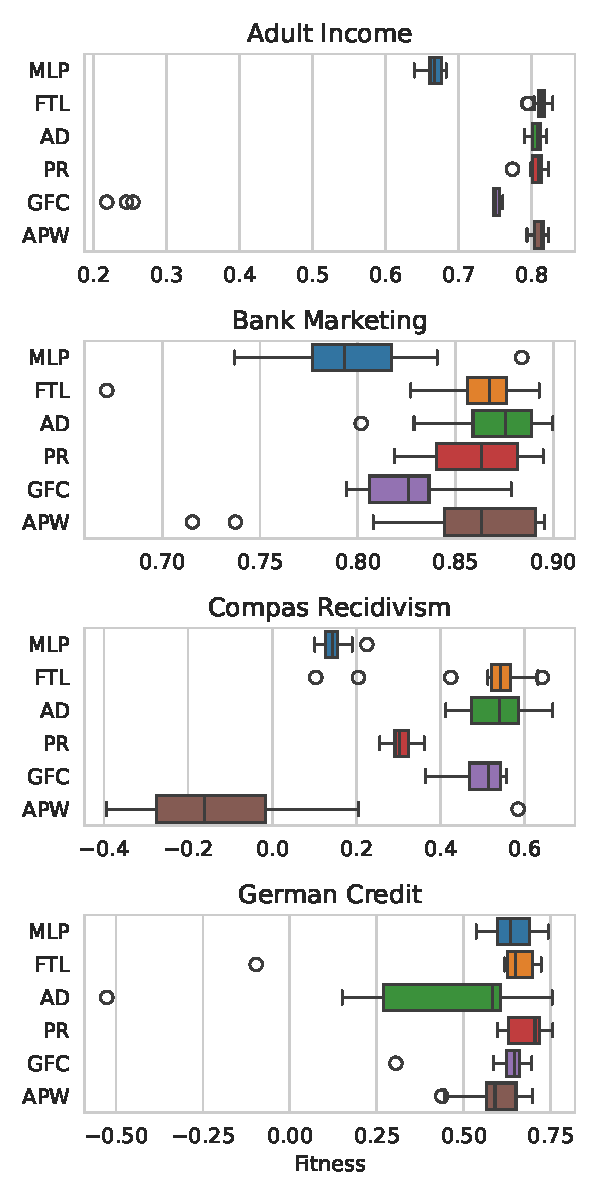
\includegraphics[width=1\linewidth]{images/boxplot_acc_parity.pdf}
\end{subfigure}
\begin{subfigure}{.32\linewidth}
    \caption{Equal Opportunity}
    \label{fig:boxplot_acc_opp}
    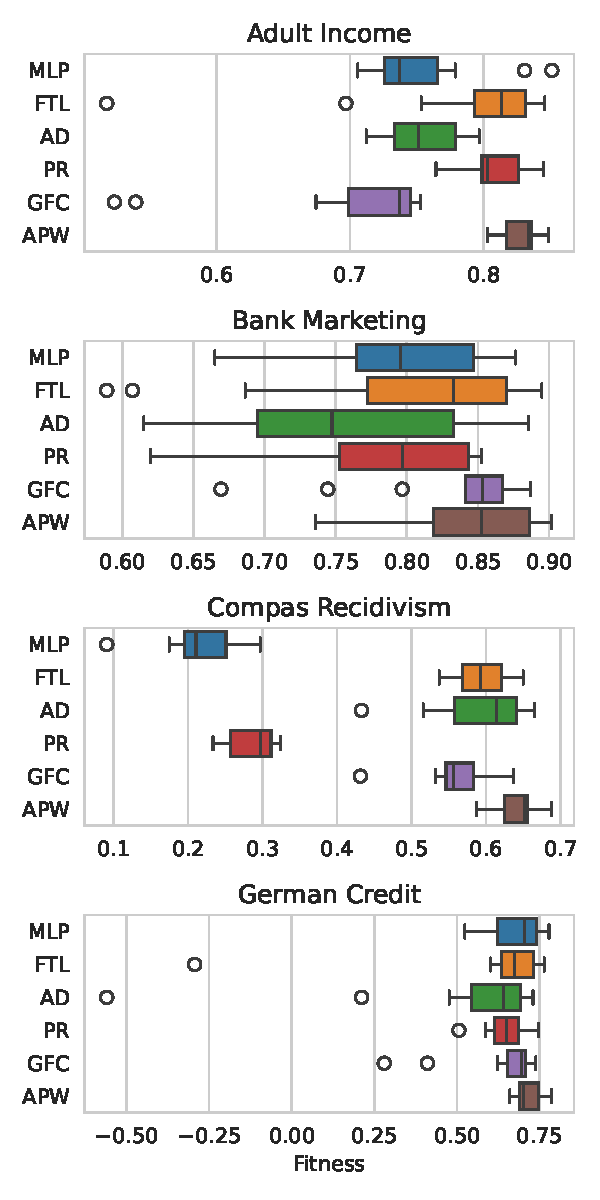
\includegraphics[width=1\linewidth]{images/boxplot_acc_opportunity.pdf}
\end{subfigure}
\begin{subfigure}{.32\linewidth}
    \caption{Equalized Odds}
    \label{fig:boxplot_acc_odds}
    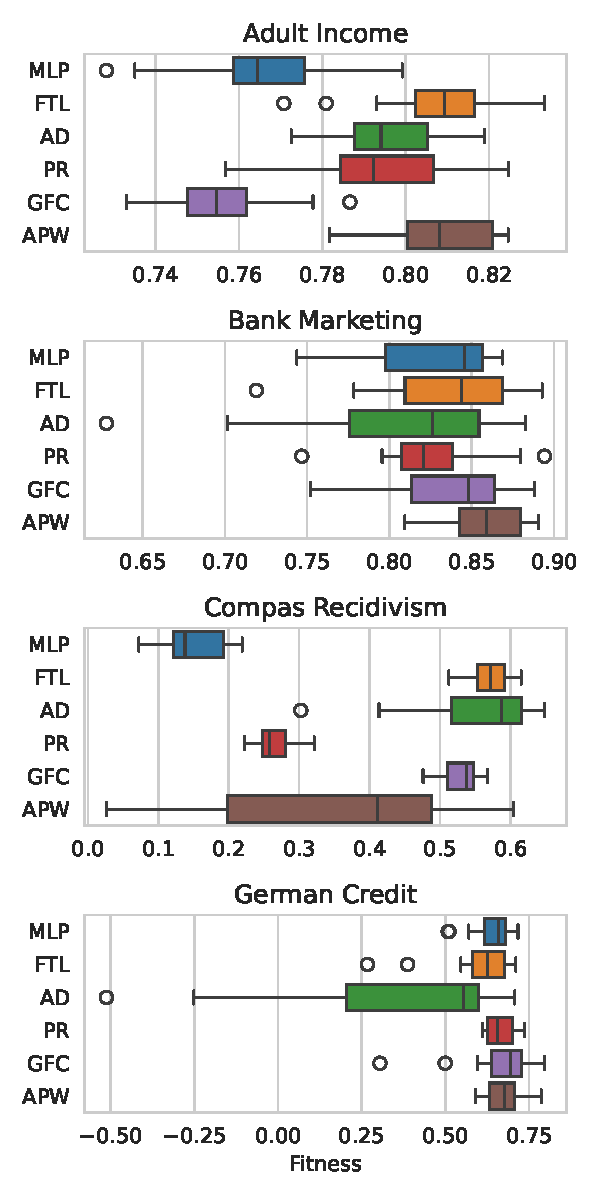
\includegraphics[width=1\linewidth]{images/boxplot_acc_odds.pdf}
\end{subfigure}
\end{figure}

Fair Transition Loss consistently demonstrates effective bias mitigation, it does so by absorbing the nuances of the dataset and the fairness metric through its transition matrices, resulting in stochastically superior fitness values in a significant number of scenarios. Additionally, the method has the capacity to effectively handle datasets with unbalanced classes when optimizing for metrics like MCC. However, it's important to recognize that Fair Transition Loss requires fine-tuning multiple hyperparameters. We thus consider that this technique is especially beneficial in setups where hyperparameter optimization is an inherent part of the prediction pipeline.

A key concern is about the potential for fairness-promoting techniques to inadvertently shift the burden onto the very group they aim to protect. This arises from the possibility that by imposing additional constraints, the method might unintentionally learn alternative ways to reproduce and even reinforce the negative social biases present in the data, thus harming the individuals it intends to safeguard.

\begin{figure}[!ht]
\centering
\caption{Results of false negatives and false positives within groups on protected promotion ($p_1$) parameter at increasing levels.}
    \label{fig:ftl_sensibility_test}
    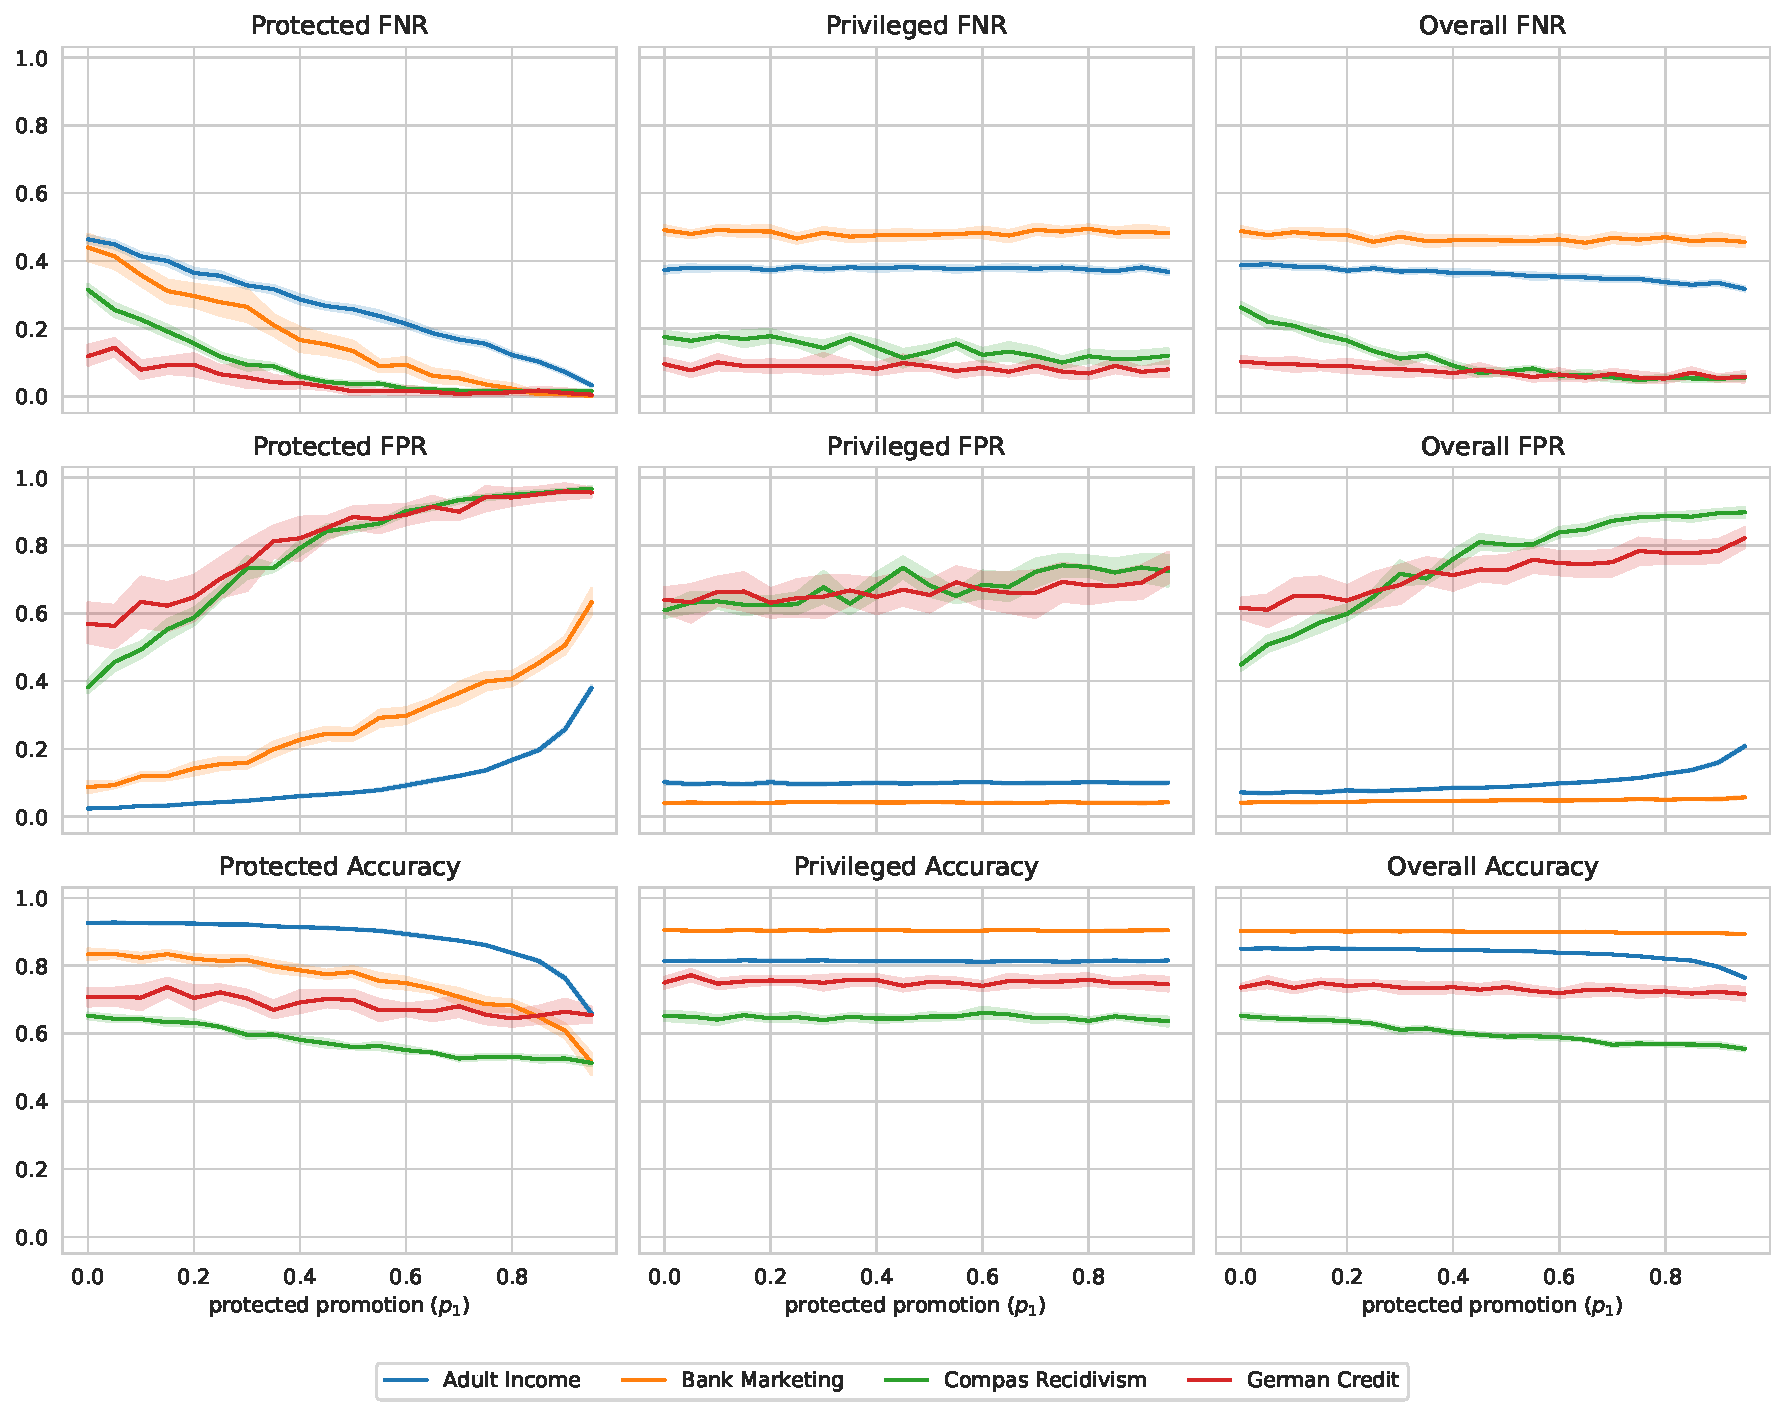
\includegraphics[width=1\linewidth]{images/ftl_sensibility_results.pdf}
\end{figure}

To evaluate the capability of FTL to address this risk, we present another experiment, where we adjusted only the protected promotion hyperparameter ($p_1$,  Equation~\ref{eq:transition_matrices}) during the FTL training, keeping all other FTL hyperparameters at zero and dropout at $0.2$. Here we follow the same re-sampling procedure, each experiment is performed over $15$ repetitions, shuffling the dataset before splitting. This experiment was conducted using the four datasets previously analyzed, and we reported the following metrics assessed over the training set: protected false negative rate, protected false positive rate, protected accuracy, privileged false negative rate, privileged false positive rate, privileged accuracy, overall false negative rate, overall false positive rate and overall accuracy.

The results, presented in Figure~\ref{fig:ftl_sensibility_test}, show that increasing the protected promotion hyperparameter value leads to a decreased false negative rate for the protected group. Meanwhile, most other monitored metrics tended towards stability to reasonable hyperparameter levels ($p_1$ under $0.95$) . An exception is the false positive rate, specially to protected group, which increased as the false negative rate decreased to keep accuracy. This pattern was consistent across all evaluated datasets. The primary aim of this experiment was to demonstrate that our proposed technique does not inadvertently penalize the protected group. Rather, the overall impact of increasing the aforementioned parameter is to effectively promote fairness for the protected group without detriment to either the privileged or protected groups. The behavior of the remaining FTL parameters is analogous, necessitating proper fine-tuning to achieve a balanced outcome. This underscores the efficacy of our method in achieving its intended purpose of reducing bias and promoting fairness in the model.

Additionally, we present performance and fairness results along with the fitness, in order to provide material to a trade-off analysis. Also, those metric values enable the reader to compare this results with different experimental setup and fitness objective from literature. Results corresponding each optimization scenario can be found on tables \ref{tab:complete_mcc_parity} to \ref{tab:complete_acc_odds}, presenting metric means and standard deviation values across multiple resample run. Best result of each metric within evaluation scenario are in bold, and standard deviation values are presented between parenthesis. Up arrow ($\uparrow$) indicates that the referred metric should be maximized while down arrow ($\downarrow$) that the metric should be minimized. To provide a visual resource to this comparison, the distribution of those metrics across multiple resample runs comparing the propose method (FTL) with baseline (MLP) and current state-of-art (APW) are presented in joint plot format in figures \ref{fig:complete_mcc_parity} to \ref{fig:complete_acc_odds}. Here each joint plot is present within the corresponding table to a better comprehension.

\newpage

\begin{table}
    \centering
    \caption{Mean and standard deviation metric values optimizing MCC and Statistical Parity in comparison with Fair Transition Loss across multiple resample runs.}\label{tab:complete_mcc_parity}
    {\scriptsize\begin{tabular}{llrrr}
    \toprule
    Dataset & Method & $\uparrow\;$Fitness & $\uparrow\;$MCC & $\downarrow\;$Stat. Parity \\
    \midrule

    \multirow{5}{*}{\shortstack[l]{Adult\\ Income}}
& Adaptive Priority Reweighting & $\textbf{0.499} \; (\pm0.01)$ & $0.510 \; (\pm0.01)$ & $0.011 \; (\pm0.01)$ \\
 & Adversarial Debiasing & $0.478 \; (\pm0.01)$ & $0.501 \; (\pm0.02)$ & $0.024 \; (\pm0.02)$ \\
 & Fair Transition Loss & $0.492 \; (\pm0.02)$ & $0.512 \; (\pm0.01)$ & $0.020 \; (\pm0.01)$ \\
 & Gerry Fair Classifier & $0.357 \; (\pm0.02)$ & $0.512 \; (\pm0.02)$ & $0.154 \; (\pm0.03)$ \\
 & Prejudice Remover & $0.491 \; (\pm0.01)$ & $0.500 \; (\pm0.01)$ & $\textbf{0.009} \; (\pm0.01)$ \\
 & Standard MLP (baseline) & $0.395 \; (\pm0.01)$ & $\textbf{0.581} \; (\pm0.01)$ & $0.185 \; (\pm0.01)$ \\
\midrule

    \multirow{5}{*}{\shortstack[l]{Bank\\ Marketing}}
& Adaptive Priority Reweighting & $0.441 \; (\pm0.03)$ & $0.482 \; (\pm0.02)$ & $0.041 \; (\pm0.04)$ \\
 & Adversarial Debiasing & $0.459 \; (\pm0.03)$ & $0.505 \; (\pm0.02)$ & $0.046 \; (\pm0.02)$ \\
 & Fair Transition Loss & $\textbf{0.539} \; (\pm0.03)$ & $\textbf{0.579} \; (\pm0.01)$ & $0.040 \; (\pm0.03)$ \\
 & Gerry Fair Classifier & $0.358 \; (\pm0.04)$ & $0.428 \; (\pm0.02)$ & $0.070 \; (\pm0.03)$ \\
 & Prejudice Remover & $0.454 \; (\pm0.03)$ & $0.487 \; (\pm0.02)$ & $\textbf{0.033} \; (\pm0.02)$ \\
 & Standard MLP (baseline) & $0.419 \; (\pm0.04)$ & $0.522 \; (\pm0.02)$ & $0.102 \; (\pm0.03)$ \\
\midrule

    \multirow{5}{*}{\shortstack[l]{COMPAS\\ Recidivism}}
& Adaptive Priority Reweighting & $-0.412 \; (\pm0.35)$ & $0.194 \; (\pm0.07)$ & $0.606 \; (\pm0.29)$ \\
 & Adversarial Debiasing & $0.157 \; (\pm0.14)$ & $\textbf{0.322} \; (\pm0.02)$ & $0.165 \; (\pm0.14)$ \\
 & Fair Transition Loss & $\textbf{0.220} \; (\pm0.06)$ & $0.276 \; (\pm0.03)$ & $0.057 \; (\pm0.05)$ \\
 & Gerry Fair Classifier & $0.141 \; (\pm0.04)$ & $0.289 \; (\pm0.06)$ & $0.148 \; (\pm0.06)$ \\
 & Prejudice Remover & $-0.318 \; (\pm0.05)$ & $-0.276 \; (\pm0.03)$ & $\textbf{0.042} \; (\pm0.03)$ \\
 & Standard MLP (baseline) & $-0.511 \; (\pm0.05)$ & $-0.299 \; (\pm0.03)$ & $0.212 \; (\pm0.04)$ \\
\midrule

    \multirow{5}{*}{\shortstack[l]{German\\ Credit}}
& Adaptive Priority Reweighting & $0.217 \; (\pm0.09)$ & $0.321 \; (\pm0.05)$ & $0.105 \; (\pm0.06)$ \\
 & Adversarial Debiasing & $0.200 \; (\pm0.17)$ & $\textbf{0.368} \; (\pm0.06)$ & $0.168 \; (\pm0.15)$ \\
 & Fair Transition Loss & $\textbf{0.272} \; (\pm0.08)$ & $0.354 \; (\pm0.07)$ & $0.083 \; (\pm0.04)$ \\
 & Gerry Fair Classifier & $0.221 \; (\pm0.09)$ & $0.291 \; (\pm0.11)$ & $\textbf{0.071} \; (\pm0.06)$ \\
 & Prejudice Remover & $0.234 \; (\pm0.09)$ & $0.329 \; (\pm0.05)$ & $0.095 \; (\pm0.06)$ \\
 & Standard MLP (baseline) & $0.223 \; (\pm0.10)$ & $0.330 \; (\pm0.07)$ & $0.107 \; (\pm0.07)$ \\
     \bottomrule
\end{tabular}}
\end{table}

\begin{figure}
\centering
\caption{Metric distribution optimizing MCC and Statistical Parity in comparison with Fair Transition Loss across multiple resample runs. Corresponding values available at Table~\ref{tab:complete_mcc_parity}.}
\label{fig:complete_mcc_parity}
\begin{subfigure}{.45\linewidth}
    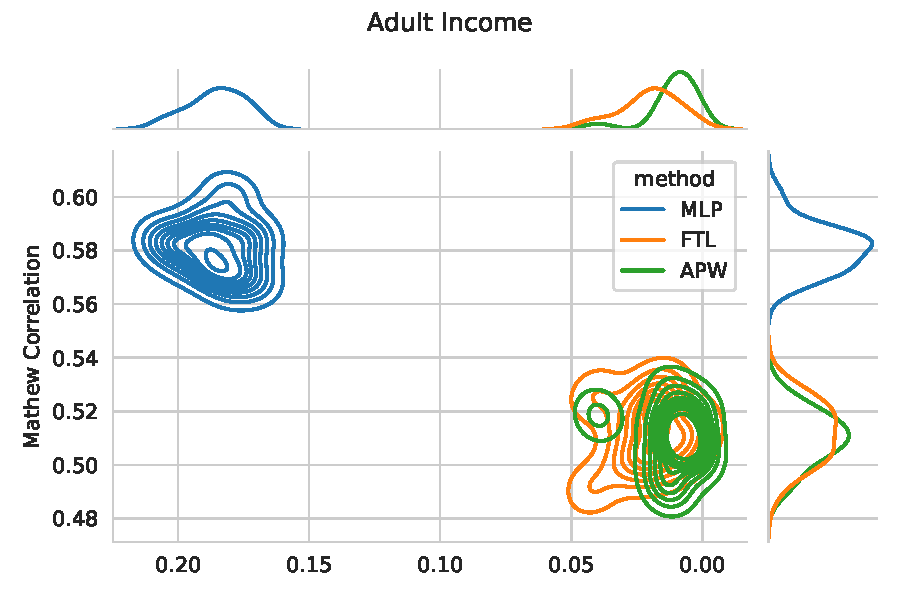
\includegraphics[width=1\linewidth]{images/pareto_mcc_parity_adult.pdf}
\end{subfigure}
\begin{subfigure}{.45\linewidth}
    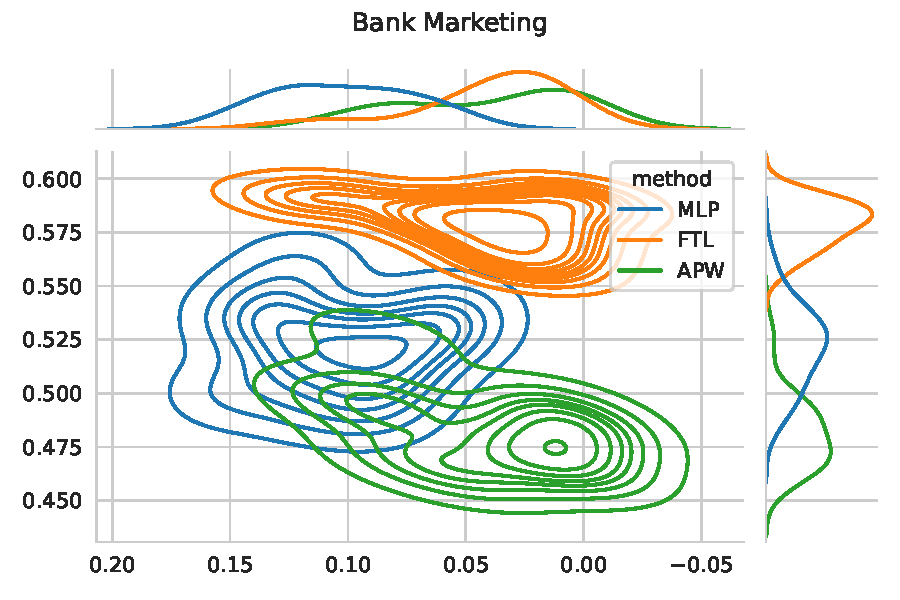
\includegraphics[width=1\linewidth]{images/pareto_mcc_parity_bank.pdf}
\end{subfigure}

\begin{subfigure}{.45\linewidth}
    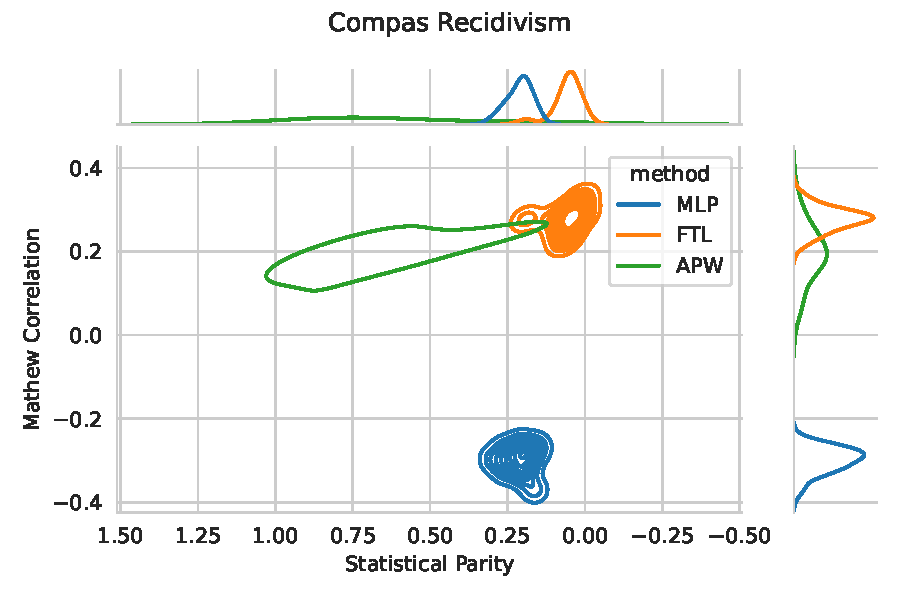
\includegraphics[width=1\linewidth]{images/pareto_mcc_parity_compas.pdf}
\end{subfigure}
\begin{subfigure}{.45\linewidth}
    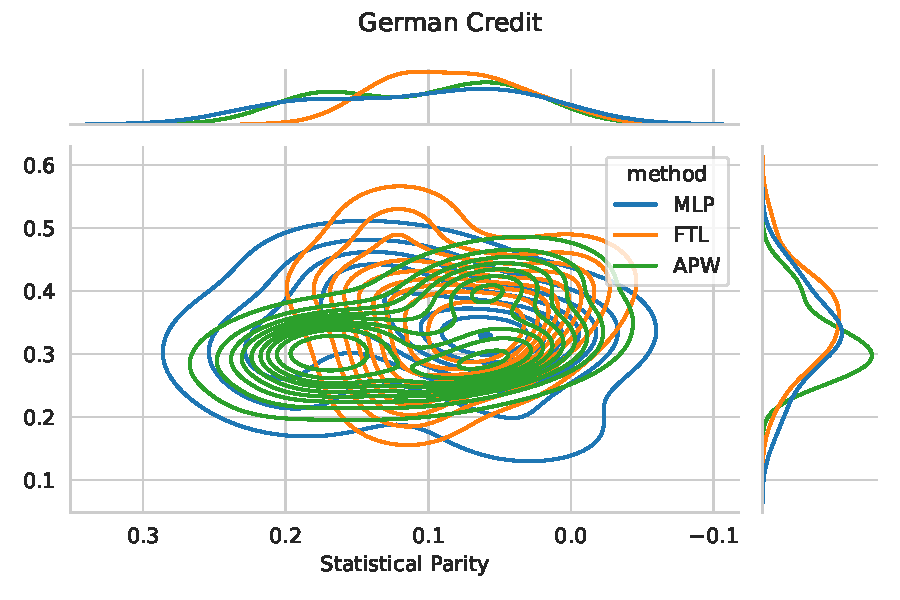
\includegraphics[width=1\linewidth]{images/pareto_mcc_parity_german.pdf}
\end{subfigure}
\end{figure}
    
 \begin{table}
    \centering
    \caption{Mean and standard deviation metric values optimizing MCC and Equal Opportunity in comparison with Fair Transition Loss across multiple resample runs.}\label{tab:complete_mcc_opportunity}
    {\scriptsize\begin{tabular}{llrrr}
    \toprule
    Dataset & Method & $\uparrow\;$Fitness & $\uparrow\;$MCC & $\downarrow\;$q. Opp. \\
    \midrule

    \multirow{5}{*}{\shortstack[l]{Adult\\ Income}}
& Adaptive Priority Reweighting & $0.493 \; (\pm0.01)$ & $0.523 \; (\pm0.01)$ & $\textbf{0.030} \; (\pm0.01)$ \\
 & Adversarial Debiasing & $0.509 \; (\pm0.03)$ & $0.565 \; (\pm0.02)$ & $0.056 \; (\pm0.02)$ \\
 & Fair Transition Loss & $\textbf{0.523} \; (\pm0.02)$ & $\textbf{0.576} \; (\pm0.02)$ & $0.052 \; (\pm0.02)$ \\
 & Gerry Fair Classifier & $0.434 \; (\pm0.01)$ & $0.523 \; (\pm0.01)$ & $0.089 \; (\pm0.01)$ \\
 & Prejudice Remover & $0.509 \; (\pm0.05)$ & $0.558 \; (\pm0.02)$ & $0.049 \; (\pm0.03)$ \\
 & Standard MLP (baseline) & $0.489 \; (\pm0.03)$ & $0.576 \; (\pm0.01)$ & $0.087 \; (\pm0.03)$ \\
\midrule

    \multirow{5}{*}{\shortstack[l]{Bank\\ Marketing}}
& Adaptive Priority Reweighting & $0.424 \; (\pm0.04)$ & $0.474 \; (\pm0.02)$ & $\textbf{0.050} \; (\pm0.04)$ \\
 & Adversarial Debiasing & $0.426 \; (\pm0.06)$ & $0.512 \; (\pm0.02)$ & $0.086 \; (\pm0.05)$ \\
 & Fair Transition Loss & $\textbf{0.485} \; (\pm0.06)$ & $\textbf{0.569} \; (\pm0.01)$ & $0.084 \; (\pm0.06)$ \\
 & Gerry Fair Classifier & $0.371 \; (\pm0.04)$ & $0.423 \; (\pm0.02)$ & $0.052 \; (\pm0.03)$ \\
 & Prejudice Remover & $0.413 \; (\pm0.04)$ & $0.485 \; (\pm0.02)$ & $0.072 \; (\pm0.04)$ \\
 & Standard MLP (baseline) & $0.439 \; (\pm0.03)$ & $0.514 \; (\pm0.02)$ & $0.075 \; (\pm0.03)$ \\
\midrule

    \multirow{5}{*}{\shortstack[l]{COMPAS\\ Recidivism}}
& Adaptive Priority Reweighting & $-0.111 \; (\pm0.18)$ & $0.260 \; (\pm0.04)$ & $0.371 \; (\pm0.17)$ \\
 & Adversarial Debiasing & $0.191 \; (\pm0.11)$ & $\textbf{0.324} \; (\pm0.03)$ & $0.133 \; (\pm0.10)$ \\
 & Fair Transition Loss & $\textbf{0.208} \; (\pm0.06)$ & $0.283 \; (\pm0.02)$ & $0.074 \; (\pm0.05)$ \\
 & Gerry Fair Classifier & $0.155 \; (\pm0.05)$ & $0.274 \; (\pm0.06)$ & $0.120 \; (\pm0.04)$ \\
 & Prejudice Remover & $-0.352 \; (\pm0.03)$ & $-0.278 \; (\pm0.02)$ & $\textbf{0.073} \; (\pm0.03)$ \\
 & Standard MLP (baseline) & $-0.471 \; (\pm0.05)$ & $-0.294 \; (\pm0.02)$ & $0.176 \; (\pm0.04)$ \\
\midrule

    \multirow{5}{*}{\shortstack[l]{German\\ Credit}}
& Adaptive Priority Reweighting & $\textbf{0.299} \; (\pm0.08)$ & $0.373 \; (\pm0.06)$ & $\textbf{0.075} \; (\pm0.05)$ \\
 & Adversarial Debiasing & $0.040 \; (\pm0.41)$ & $0.301 \; (\pm0.13)$ & $0.261 \; (\pm0.30)$ \\
 & Fair Transition Loss & $0.273 \; (\pm0.10)$ & $0.386 \; (\pm0.08)$ & $0.113 \; (\pm0.08)$ \\
 & Gerry Fair Classifier & $0.218 \; (\pm0.11)$ & $0.321 \; (\pm0.10)$ & $0.103 \; (\pm0.05)$ \\
 & Prejudice Remover & $0.283 \; (\pm0.10)$ & $\textbf{0.391} \; (\pm0.07)$ & $0.107 \; (\pm0.06)$ \\
 & Standard MLP (baseline) & $0.270 \; (\pm0.07)$ & $0.352 \; (\pm0.05)$ & $0.082 \; (\pm0.04)$ \\
     \bottomrule
\end{tabular}}
\end{table}

\begin{figure}
\centering
\caption{Metric distribution optimizing MCC and Equal Opportunity in comparison with Fair Transition Loss across multiple resample runs. Corresponding values available at Table~\ref{tab:complete_mcc_opportunity}.}
\label{fig:complete_mcc_opportunity}
\begin{subfigure}{.45\linewidth}
    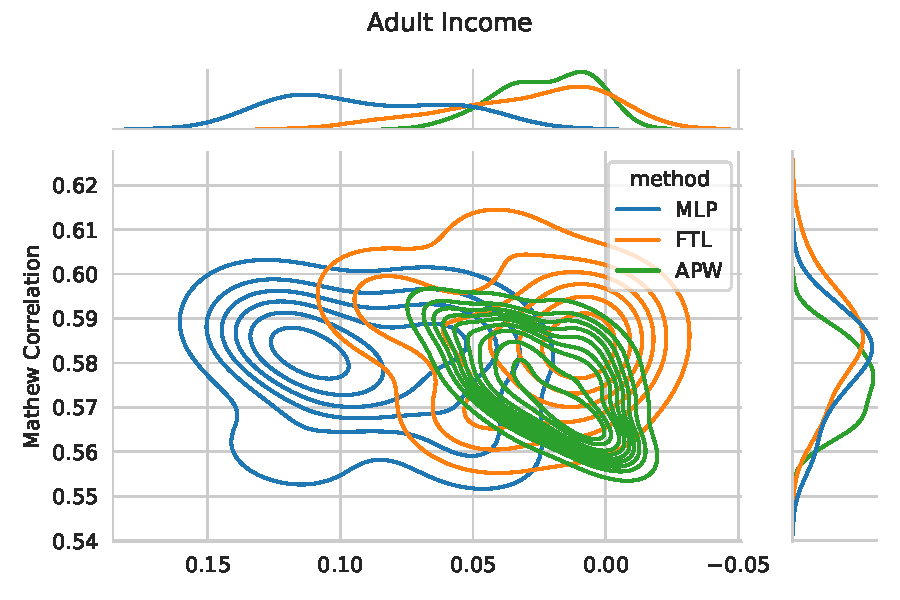
\includegraphics[width=1\linewidth]{images/pareto_mcc_opportunity_adult.pdf}
\end{subfigure}
\begin{subfigure}{.45\linewidth}
    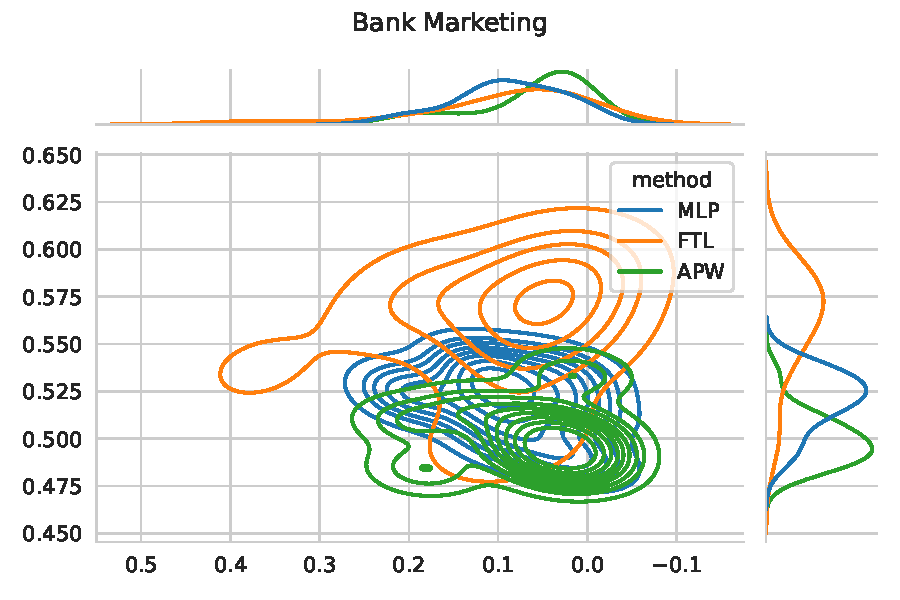
\includegraphics[width=1\linewidth]{images/pareto_mcc_opportunity_bank.pdf}
\end{subfigure}

\begin{subfigure}{.45\linewidth}
    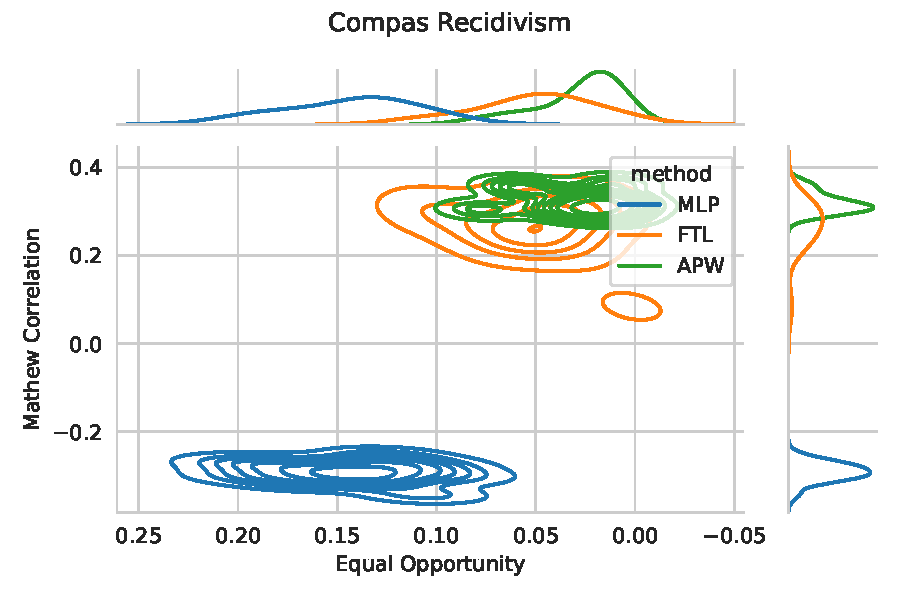
\includegraphics[width=1\linewidth]{images/pareto_mcc_opportunity_compas.pdf}
\end{subfigure}
\begin{subfigure}{.45\linewidth}
    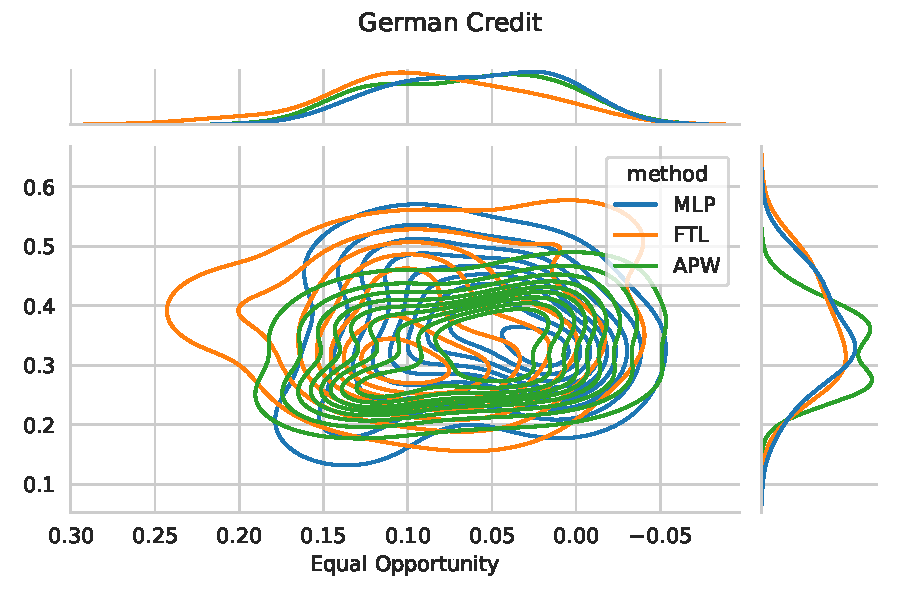
\includegraphics[width=1\linewidth]{images/pareto_mcc_opportunity_german.pdf}
\end{subfigure}
\end{figure}

 \begin{table}
    \centering
    \caption{Mean and standard deviation metric values optimizing MCC and Equalized Odds in comparison with Fair Transition Loss across multiple resample runs.}\label{tab:complete_mcc_odds}
    {\scriptsize\begin{tabular}{llrrr}
    \toprule
    Dataset & Method & $\uparrow\;$Fitness & $\uparrow\;$MCC & $\downarrow\;$Eq. Odds \\
    \midrule

    \multirow{5}{*}{\shortstack[l]{Adult\\ Income}}
& Adaptive Priority Reweighting & $0.553 \; (\pm0.01)$ & $0.576 \; (\pm0.01)$ & $\textbf{0.022} \; (\pm0.02)$\\
 & Adversarial Debiasing & $0.493 \; (\pm0.05)$ & $0.573 \; (\pm0.01)$ & $0.080 \; (\pm0.05)$ \\
 & Fair Transition Loss & $\textbf{0.556} \; (\pm0.03)$& $\textbf{0.584} \; (\pm0.01)$& $0.029 \; (\pm0.03)$ \\
 & Gerry Fair Classifier & $0.394 \; (\pm0.03)$ & $0.515 \; (\pm0.02)$ & $0.121 \; (\pm0.02)$ \\
 & Prejudice Remover & $0.505 \; (\pm0.09)$ & $0.560 \; (\pm0.02)$ & $0.055 \; (\pm0.08)$ \\
 & Standard MLP (baseline) & $0.489 \; (\pm0.03)$ & $0.580 \; (\pm0.01)$ & $0.091 \; (\pm0.03)$ \\
\midrule

    \multirow{5}{*}{\shortstack[l]{Bank\\ Marketing}}
& Adaptive Priority Reweighting & $0.441 \; (\pm0.06)$ & $0.500 \; (\pm0.01)$ & $\textbf{0.059} \; (\pm0.06)$\\
 & Adversarial Debiasing & $0.373 \; (\pm0.09)$ & $0.508 \; (\pm0.02)$ & $0.136 \; (\pm0.09)$ \\
 & Fair Transition Loss & $\textbf{0.467} \; (\pm0.11)$& $0.560 \; (\pm0.03)$ & $0.093 \; (\pm0.10)$ \\
 & Gerry Fair Classifier & $0.344 \; (\pm0.07)$ & $0.422 \; (\pm0.02)$ & $0.078 \; (\pm0.06)$ \\
 & Prejudice Remover & $0.392 \; (\pm0.09)$ & $0.490 \; (\pm0.02)$ & $0.098 \; (\pm0.08)$ \\
 & Standard MLP (baseline) & $0.432 \; (\pm0.06)$ & $\textbf{0.520} \; (\pm0.02)$& $0.087 \; (\pm0.06)$ \\
\midrule

    \multirow{5}{*}{\shortstack[l]{COMPAS\\ Recidivism}}
& Adaptive Priority Reweighting & $\textbf{0.292} \; (\pm0.03)$& $0.319 \; (\pm0.02)$ & $\textbf{0.027} \; (\pm0.02)$\\
 & Adversarial Debiasing & $0.258 \; (\pm0.05)$ & $\textbf{0.329} \; (\pm0.03)$& $0.070 \; (\pm0.05)$ \\
 & Fair Transition Loss & $0.213 \; (\pm0.06)$ & $0.264 \; (\pm0.06)$ & $0.050 \; (\pm0.03)$ \\
 & Gerry Fair Classifier & $0.201 \; (\pm0.05)$ & $0.290 \; (\pm0.04)$ & $0.089 \; (\pm0.05)$ \\
 & Prejudice Remover & $-0.319 \; (\pm0.03)$ & $-0.289 \; (\pm0.03)$ & $0.030 \; (\pm0.02)$ \\
 & Standard MLP (baseline) & $-0.435 \; (\pm0.03)$ & $-0.292 \; (\pm0.02)$ & $0.143 \; (\pm0.03)$ \\
\midrule

    \multirow{5}{*}{\shortstack[l]{German\\ Credit}}
& Adaptive Priority Reweighting & $0.261 \; (\pm0.08)$ & $0.326 \; (\pm0.06)$ & $0.065 \; (\pm0.05)$ \\
 & Adversarial Debiasing & $0.116 \; (\pm0.40)$ & $0.311 \; (\pm0.14)$ & $0.195 \; (\pm0.28)$ \\
 & Fair Transition Loss & $0.274 \; (\pm0.10)$ & $\textbf{0.361} \; (\pm0.08)$& $0.087 \; (\pm0.05)$ \\
 & Gerry Fair Classifier & $0.273 \; (\pm0.10)$ & $\textbf{0.361} \; (\pm0.06)$& $0.087 \; (\pm0.06)$ \\
 & Prejudice Remover & $0.271 \; (\pm0.07)$ & $0.324 \; (\pm0.06)$ & $\textbf{0.054} \; (\pm0.04)$\\
 & Standard MLP (baseline) & $\textbf{0.295} \; (\pm0.09)$& $0.354 \; (\pm0.08)$ & $0.060 \; (\pm0.04)$ \\
     \bottomrule
\end{tabular}}
\end{table}

\begin{figure}
\centering
\caption{Metric distribution optimizing MCC and Equalized Odds in comparison with Fair Transition Loss across multiple resample runs. Corresponding values available at Table~\ref{tab:complete_mcc_odds}.}
\label{fig:complete_mcc_odds}
\begin{subfigure}{.45\linewidth}
    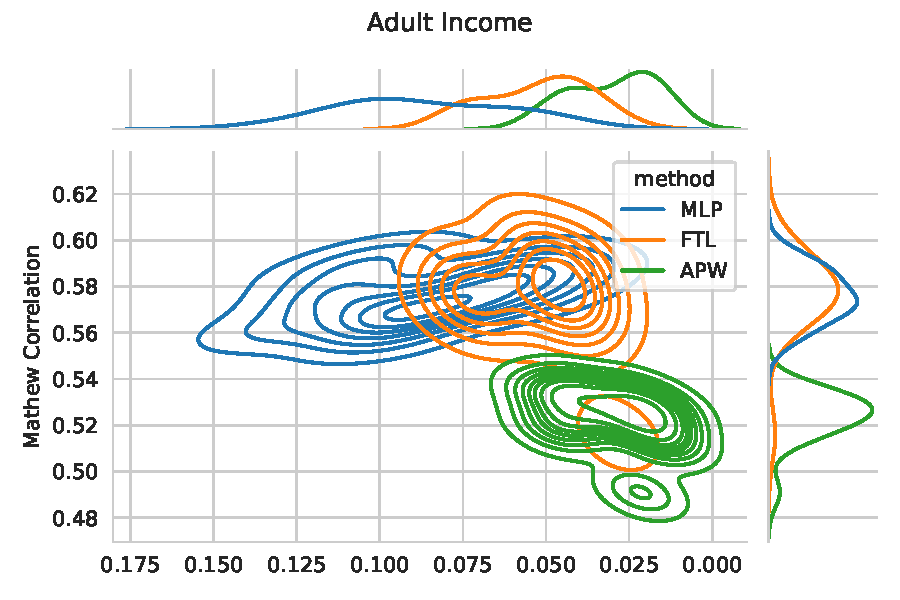
\includegraphics[width=1\linewidth]{images/pareto_mcc_odds_adult.pdf}
\end{subfigure}
\begin{subfigure}{.45\linewidth}
    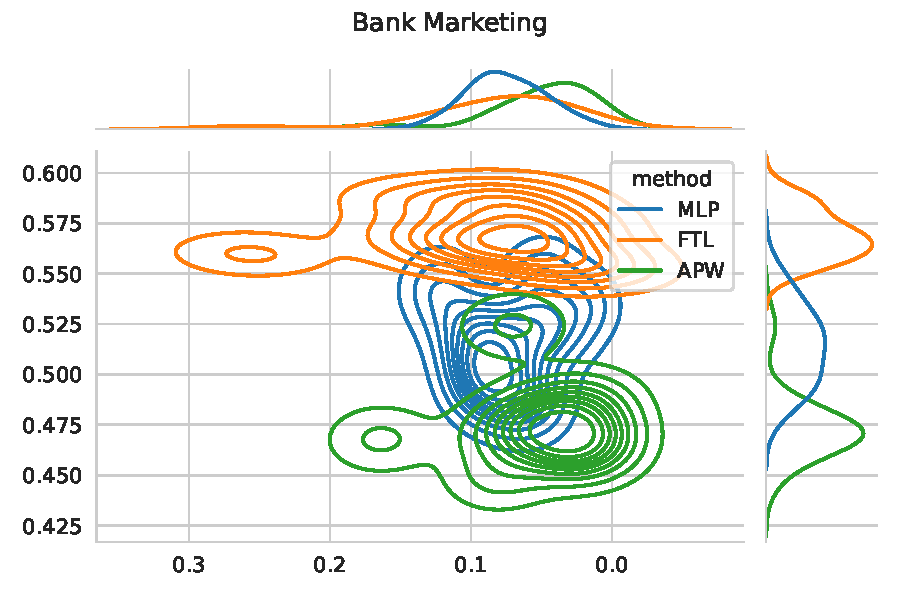
\includegraphics[width=1\linewidth]{images/pareto_mcc_odds_bank.pdf}
\end{subfigure}

\begin{subfigure}{.45\linewidth}
    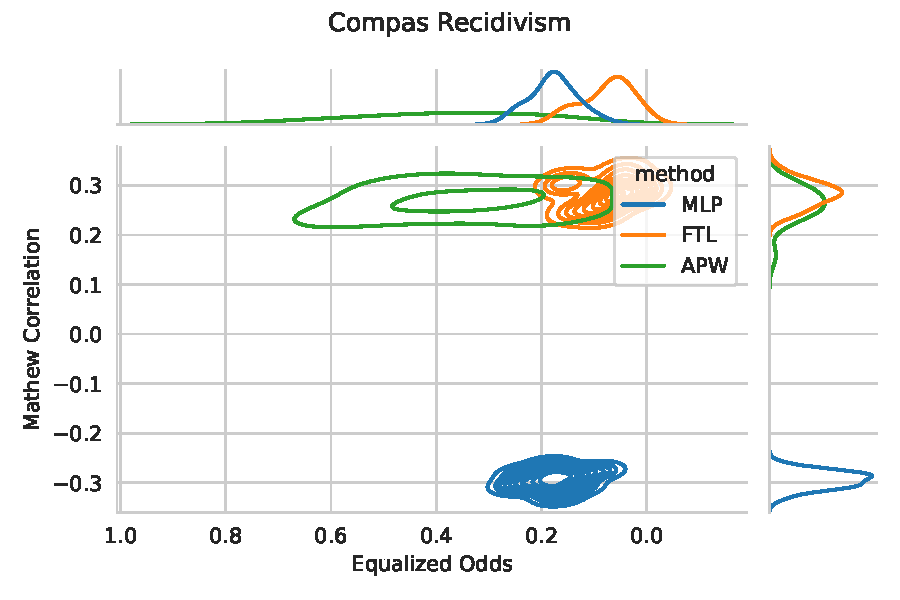
\includegraphics[width=1\linewidth]{images/pareto_mcc_odds_compas.pdf}
\end{subfigure}
\begin{subfigure}{.45\linewidth}
    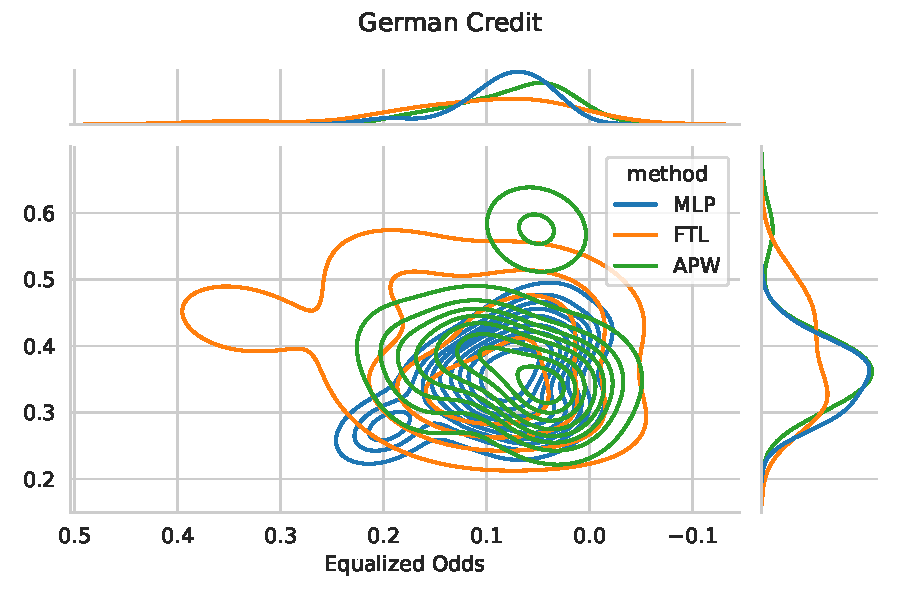
\includegraphics[width=1\linewidth]{images/pareto_mcc_odds_german.pdf}
\end{subfigure}
\end{figure}


 \begin{table}
    \centering
    \caption{Mean and standard deviation metric values optimizing Accuracy and Statistical Parity in comparison with Fair Transition Loss across multiple resample runs.}\label{tab:complete_acc_parity}
   {\scriptsize \begin{tabular}{llrrr}
    \toprule
    Dataset & Method & $\uparrow\;$Fitness & $\uparrow\;$Accuracy & $\downarrow\;$Stat. Parity \\
    \midrule

    \multirow{5}{*}{\shortstack[l]{Adult\\ Income}}
& Adaptive Priority Reweighting & $0.811 \; (\pm0.01)$ & $0.822 \; (\pm0.01)$ & $\textbf{0.011}(\pm0.01)$\\
 & Adversarial Debiasing & $0.808 \; (\pm0.01)$ & $0.830 \; (\pm0.01)$ & $0.022 \; (\pm0.01)$ \\
 & Fair Transition Loss & $\textbf{0.814} \; (\pm0.01)$& $0.828 \; (\pm0.01)$ & $0.014 \; (\pm0.01)$ \\
 & Gerry Fair Classifier & $0.651 \; (\pm0.21)$ & $0.721 \; (\pm0.07)$ & $0.070 \; (\pm0.14)$ \\
 & Prejudice Remover & $0.807 \; (\pm0.01)$ & $0.825 \; (\pm0.00)$ & $0.018 \; (\pm0.01)$ \\
 & Standard MLP (baseline) & $0.666 \; (\pm0.01)$ & $\textbf{0.851} \; (\pm0.00)$& $0.184 \; (\pm0.01)$ \\
\midrule

    \multirow{5}{*}{\shortstack[l]{Bank\\ Marketing}}
& Adaptive Priority Reweighting & $0.851 \; (\pm0.06)$ & $0.900 \; (\pm0.00)$ & $0.049 \; (\pm0.06)$ \\
 & Adversarial Debiasing & $\textbf{0.869} \; (\pm0.03)$& $0.901 \; (\pm0.00)$ & $\textbf{0.031} \; (\pm0.02)$\\
 & Fair Transition Loss & $0.854 \; (\pm0.05)$ & $0.889 \; (\pm0.01)$ & $0.035 \; (\pm0.05)$ \\
 & Gerry Fair Classifier & $0.824 \; (\pm0.02)$ & $0.895 \; (\pm0.00)$ & $0.071 \; (\pm0.02)$ \\
 & Prejudice Remover & $0.860 \; (\pm0.02)$ & $0.898 \; (\pm0.00)$ & $0.038 \; (\pm0.02)$ \\
 & Standard MLP (baseline) & $0.799 \; (\pm0.04)$ & $\textbf{0.902} \; (\pm0.00)$& $0.103 \; (\pm0.03)$ \\
\midrule

    \multirow{5}{*}{\shortstack[l]{COMPAS\\ Recidivism}}
& Adaptive Priority Reweighting & $-0.105 \; (\pm0.26)$ & $0.584 \; (\pm0.03)$ & $0.689 \; (\pm0.23)$ \\
 & Adversarial Debiasing & $\textbf{0.538} \; (\pm0.07)$& $\textbf{0.670} \; (\pm0.02)$& $0.132 \; (\pm0.08)$ \\
 & Fair Transition Loss & $0.501 \; (\pm0.15)$ & $0.600 \; (\pm0.05)$ & $0.099 \; (\pm0.14)$ \\
 & Gerry Fair Classifier & $0.501 \; (\pm0.05)$ & $0.614 \; (\pm0.05)$ & $0.113 \; (\pm0.07)$ \\
 & Prejudice Remover & $0.308 \; (\pm0.03)$ & $0.359 \; (\pm0.01)$ & $\textbf{0.052} \; (\pm0.02)$\\
 & Standard MLP (baseline) & $0.146 \; (\pm0.03)$ & $0.354 \; (\pm0.02)$ & $0.208 \; (\pm0.02)$ \\
\midrule

    \multirow{5}{*}{\shortstack[l]{German\\ Credit}}
& Adaptive Priority Reweighting & $0.589 \; (\pm0.08)$ & $0.682 \; (\pm0.03)$ & $0.093 \; (\pm0.08)$ \\
 & Adversarial Debiasing & $0.430 \; (\pm0.33)$ & $0.713 \; (\pm0.09)$ & $0.283 \; (\pm0.26)$ \\
 & Fair Transition Loss & $0.616 \; (\pm0.20)$ & $0.715 \; (\pm0.06)$ & $0.098 \; (\pm0.17)$ \\
 & Gerry Fair Classifier & $0.621 \; (\pm0.09)$ & $0.712 \; (\pm0.12)$ & $0.090 \; (\pm0.04)$ \\
 & Prejudice Remover & $\textbf{0.684} \; (\pm0.05)$& $\textbf{0.757} \; (\pm0.02)$& $\textbf{0.073} \; (\pm0.06)$\\
 & Standard MLP (baseline) & $0.639 \; (\pm0.06)$ & $0.752 \; (\pm0.02)$ & $0.113 \; (\pm0.06)$ \\
     \bottomrule
\end{tabular}}
\end{table}


\begin{figure}
\centering
\caption{Metric distribution optimizing Accuracy and Statistical Parity in comparison with Fair Transition Loss across multiple resample runs. Corresponding values available at Table~\ref{tab:complete_acc_parity}.}
\label{fig:complete_acc_parity}
\begin{subfigure}{.45\linewidth}
    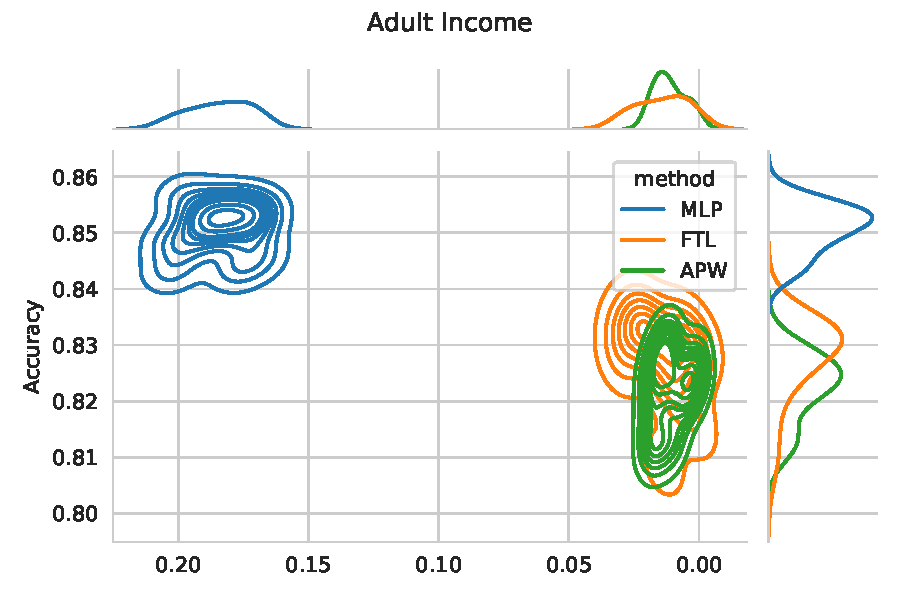
\includegraphics[width=1\linewidth]{images/pareto_acc_parity_adult.pdf}
\end{subfigure}
\begin{subfigure}{.45\linewidth}
    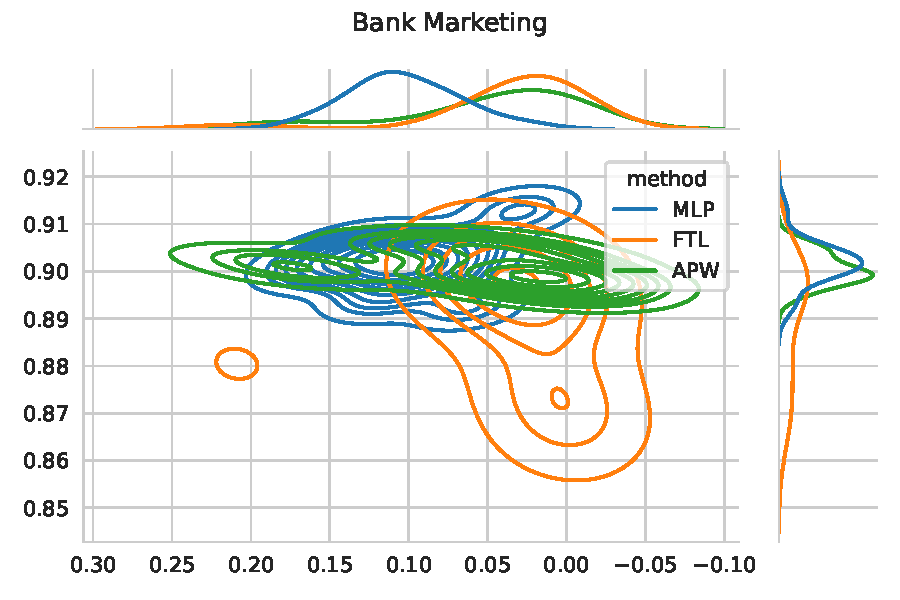
\includegraphics[width=1\linewidth]{images/pareto_acc_parity_bank.pdf}
\end{subfigure}

\begin{subfigure}{.45\linewidth}
    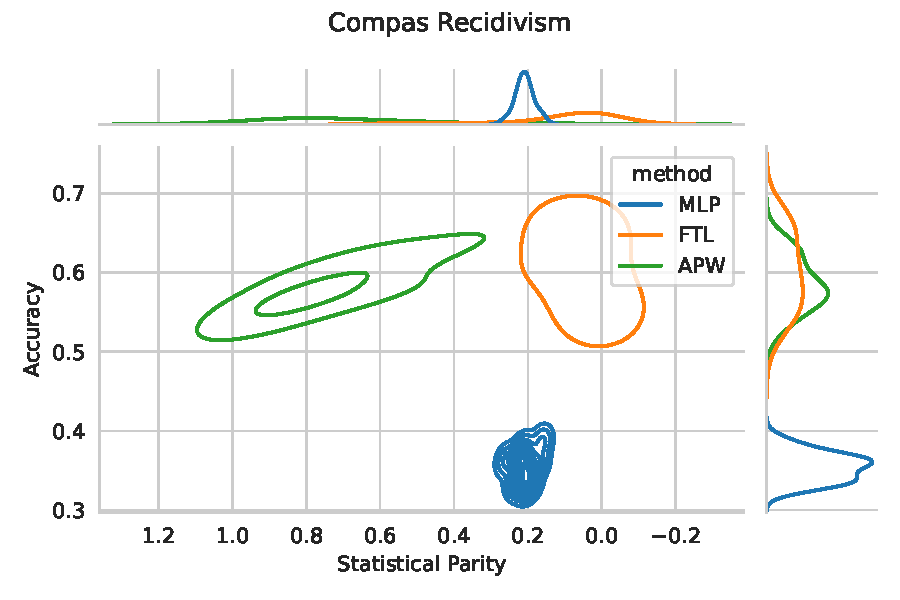
\includegraphics[width=1\linewidth]{images/pareto_acc_parity_compas.pdf}
\end{subfigure}
\begin{subfigure}{.45\linewidth}
    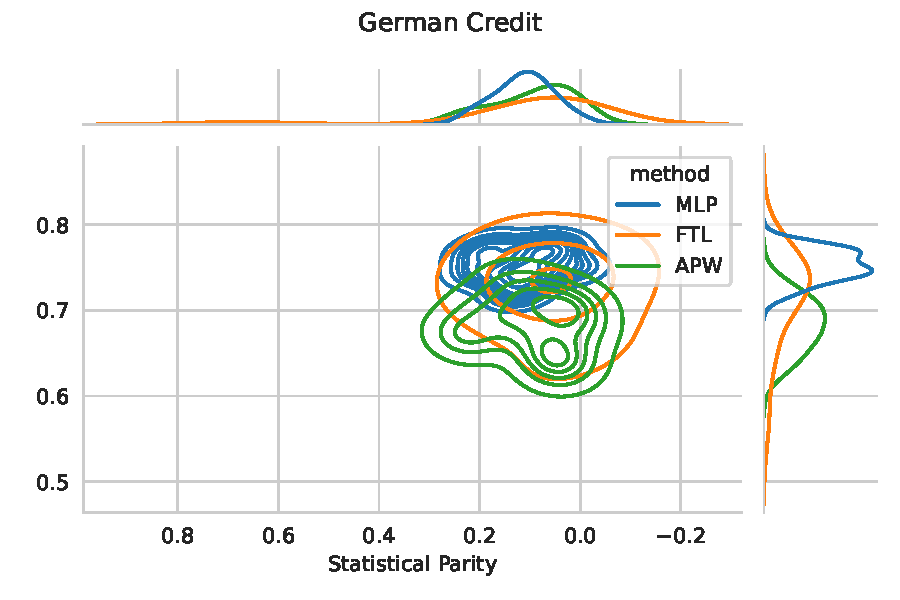
\includegraphics[width=1\linewidth]{images/pareto_acc_parity_german.pdf}
\end{subfigure}
\end{figure}

\begin{table}
    \centering
    \caption{Mean and standard deviation metric values optimizing Accuracy and Equal Opportunity in comparison with Fair Transition Loss.}\label{tab:complete_acc_opportunity}
    {\scriptsize \begin{tabular}{llrrr}
    \toprule
    Dataset & Method & $\uparrow\;$Fitness & $\uparrow\;$Accuracy & $\downarrow\;$Eq. Opp. \\
    \midrule

    \multirow{5}{*}{\shortstack[l]{Adult\\ Income}}
& Adaptive Priority Reweighting & $\textbf{0.808} \; (\pm0.01)$& $0.837 \; (\pm0.00)$ & $\textbf{0.029} \; (\pm0.01)$\\
 & Adversarial Debiasing & $0.796 \; (\pm0.01)$ & $0.849 \; (\pm0.00)$ & $0.052 \; (\pm0.01)$ \\
 & Fair Transition Loss & $0.808 \; (\pm0.02)$ & $0.842 \; (\pm0.01)$ & $0.034 \; (\pm0.02)$ \\
 & Gerry Fair Classifier & $0.756 \; (\pm0.01)$ & $0.788 \; (\pm0.03)$ & $0.032 \; (\pm0.04)$ \\
 & Prejudice Remover & $0.794 \; (\pm0.02)$ & $0.845 \; (\pm0.01)$ & $0.051 \; (\pm0.01)$ \\
 & Standard MLP (baseline) & $0.765 \; (\pm0.02)$ & $\textbf{0.850} \; (\pm0.00)$& $0.084 \; (\pm0.02)$ \\
\midrule

    \multirow{5}{*}{\shortstack[l]{Bank\\ Marketing}}
& Adaptive Priority Reweighting & $\textbf{0.858} \; (\pm0.02)$& $0.897 \; (\pm0.00)$ & $\textbf{0.039} \; (\pm0.03)$\\
 & Adversarial Debiasing & $0.807 \; (\pm0.07)$ & $\textbf{0.902} \; (\pm0.00)$& $0.095 \; (\pm0.07)$ \\
 & Fair Transition Loss & $0.833 \; (\pm0.05)$ & $0.892 \; (\pm0.01)$ & $0.059 \; (\pm0.05)$ \\
 & Gerry Fair Classifier & $0.837 \; (\pm0.04)$ & $0.895 \; (\pm0.00)$ & $0.058 \; (\pm0.04)$ \\
 & Prejudice Remover & $0.827 \; (\pm0.04)$ & $0.898 \; (\pm0.00)$ & $0.071 \; (\pm0.04)$ \\
 & Standard MLP (baseline) & $0.826 \; (\pm0.04)$ & $0.901 \; (\pm0.00)$& $0.075 \; (\pm0.04)$ \\
\midrule

    \multirow{5}{*}{\shortstack[l]{COMPAS\\ Recidivism}}
& Adaptive Priority Reweighting & $0.356 \; (\pm0.18)$ & $0.643 \; (\pm0.02)$ & $0.287 \; (\pm0.18)$ \\
 & Adversarial Debiasing & $0.553 \; (\pm0.09)$ & $\textbf{0.669} \; (\pm0.01)$& $0.116 \; (\pm0.09)$ \\
 & Fair Transition Loss & $\textbf{0.572} \; (\pm0.03)$& $0.631 \; (\pm0.04)$ & $\textbf{0.059} \; (\pm0.03)$\\
 & Gerry Fair Classifier & $0.530 \; (\pm0.03)$ & $0.637 \; (\pm0.04)$ & $0.107 \; (\pm0.05)$ \\
 & Prejudice Remover & $0.264 \; (\pm0.03)$ & $0.357 \; (\pm0.01)$ & $0.093 \; (\pm0.02)$ \\
 & Standard MLP (baseline) & $0.155 \; (\pm0.04)$ & $0.350 \; (\pm0.02)$ & $0.195 \; (\pm0.04)$ \\
\midrule

    \multirow{5}{*}{\shortstack[l]{German\\ Credit}}
& Adaptive Priority Reweighting & $\textbf{0.674} \; (\pm0.06)$& $0.750 \; (\pm0.03)$ & $0.076 \; (\pm0.04)$ \\
 & Adversarial Debiasing & $0.368 \; (\pm0.38)$ & $0.685 \; (\pm0.10)$ & $0.317 \; (\pm0.30)$ \\
 & Fair Transition Loss & $0.599 \; (\pm0.12)$ & $0.711 \; (\pm0.05)$ & $0.112 \; (\pm0.11)$ \\
 & Gerry Fair Classifier & $0.662 \; (\pm0.12)$ & $0.719 \; (\pm0.12)$ & $0.057 \; (\pm0.07)$ \\
 & Prejudice Remover & $0.664 \; (\pm0.05)$ & $\textbf{0.748} \; (\pm0.02)$& $0.084 \; (\pm0.04)$ \\
 & Standard MLP (baseline) & $0.638 \; (\pm0.06)$ & $0.738 \; (\pm0.04)$ & $0.101 \; (\pm0.05)$ \\
     \bottomrule
\end{tabular} }
\end{table}

\begin{figure}
\centering
\caption{Metric distribution optimizing Accuracy and Equal Opportunity in comparison with Fair Transition Loss across multiple resample runs. Corresponding values available at Table~\ref{tab:complete_acc_opportunity}.}
\label{fig:complete_acc_opportunity}
\begin{subfigure}{.45\linewidth}
    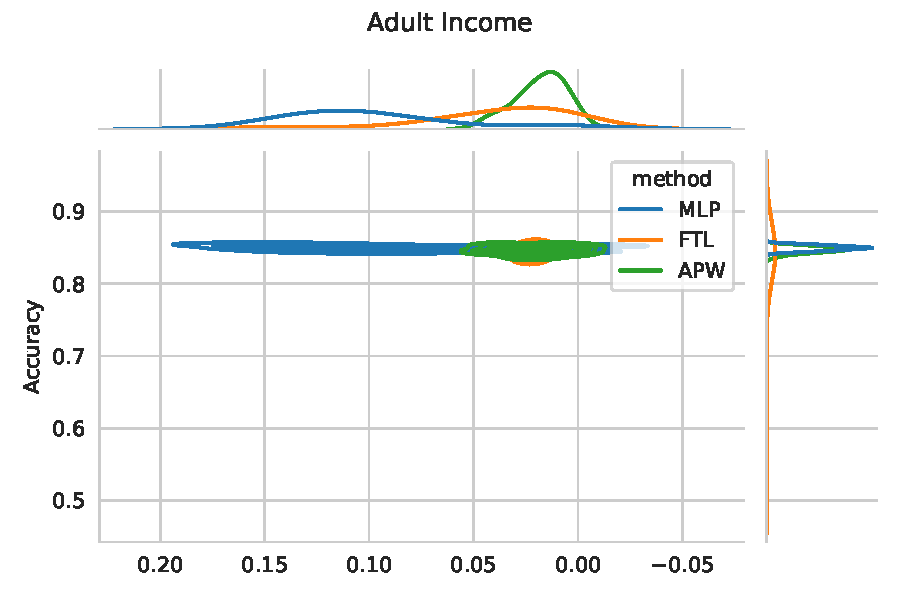
\includegraphics[width=1\linewidth]{images/pareto_acc_opportunity_adult.pdf}
\end{subfigure}
\begin{subfigure}{.45\linewidth}
    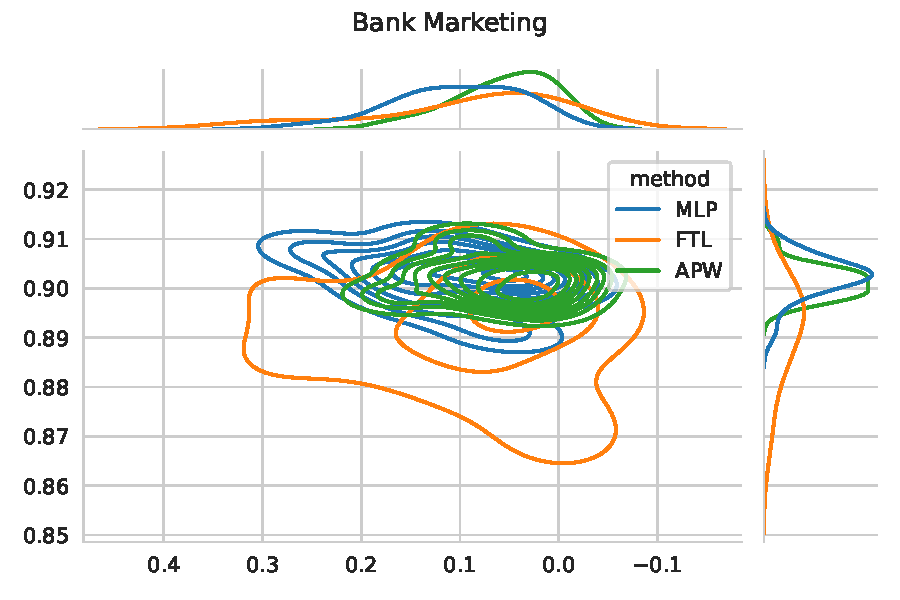
\includegraphics[width=1\linewidth]{images/pareto_acc_opportunity_bank.pdf}
\end{subfigure}

\begin{subfigure}{.45\linewidth}
    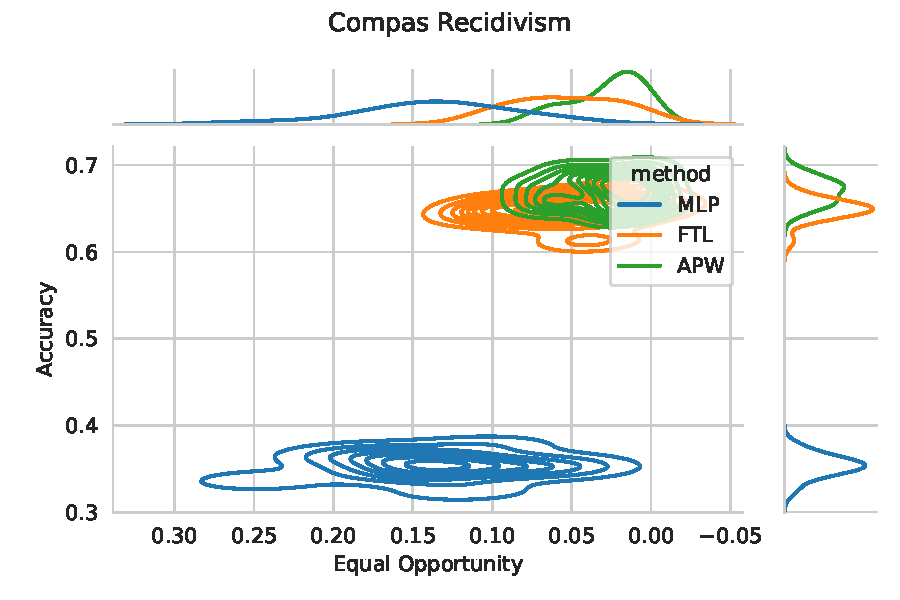
\includegraphics[width=1\linewidth]{images/pareto_acc_opportunity_compas.pdf}
\end{subfigure}
\begin{subfigure}{.45\linewidth}
    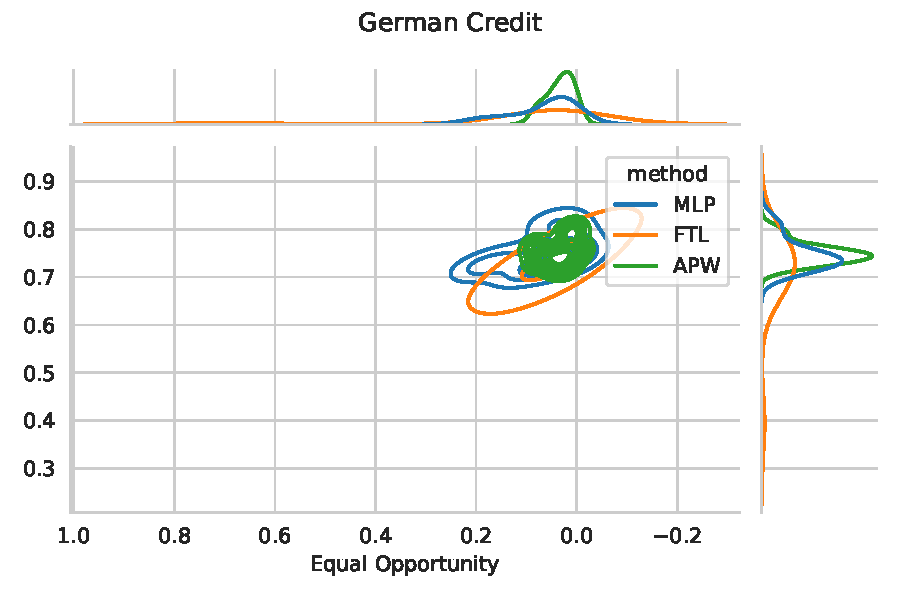
\includegraphics[width=1\linewidth]{images/pareto_acc_opportunity_german.pdf}
\end{subfigure}
\end{figure}

 \begin{table}
    \centering
    \caption{Mean and standard deviation metric values optimizing Accuracy and Equalized Odds in comparison with Fair Transition Loss across multiple resample runs.}\label{tab:complete_acc_odds}
    {\scriptsize \begin{tabular}{llrrr}
    \toprule
    Dataset & Method & $\uparrow\;$Fitness & $\uparrow\;$Accuracy & $\downarrow\;$Eq. Odds \\
    \midrule

    \multirow{5}{*}{\shortstack[l]{Adult\\ Income}}
& Adaptive Priority Reweighting & $\textbf{0.829} \; (\pm0.01)$& $0.847 \; (\pm0.00)$ & $\textbf{0.018} \; (\pm0.01)$ \\
 & Adversarial Debiasing & $0.756 \; (\pm0.03)$ & $0.848 \; (\pm0.00)$ & $0.092 \; (\pm0.03)$ \\
 & Fair Transition Loss & $0.787 \; (\pm0.08)$ & $0.826 \; (\pm0.07)$ & $0.039 \; (\pm0.04)$ \\
 & Gerry Fair Classifier & $0.705 \; (\pm0.07)$ & $0.751 \; (\pm0.09)$ & $0.046 \; (\pm0.05)$ \\
 & Prejudice Remover & $0.810 \; (\pm0.02)$ & $0.846 \; (\pm0.00)$ & $0.036 \; (\pm0.02)$ \\
 & Standard MLP (baseline) & $0.752 \; (\pm0.04)$ & $\textbf{0.849} \; (\pm0.00)$& $0.097 \; (\pm0.04)$ \\
\midrule

    \multirow{5}{*}{\shortstack[l]{Bank\\ Marketing}}
& Adaptive Priority Reweighting & $\textbf{0.846} \; (\pm0.05)$& $0.901 \; (\pm0.00)$ & $\textbf{0.055} \; (\pm0.05)$\\
 & Adversarial Debiasing & $0.750 \; (\pm0.09)$ & $0.900 \; (\pm0.00)$ & $0.150 \; (\pm0.09)$ \\
 & Fair Transition Loss & $0.799 \; (\pm0.10)$ & $0.891 \; (\pm0.01)$ & $0.092 \; (\pm0.10)$ \\
 & Gerry Fair Classifier & $0.837 \; (\pm0.06)$ & $0.893 \; (\pm0.00)$ & $0.057 \; (\pm0.06)$ \\
 & Prejudice Remover & $0.781 \; (\pm0.07)$ & $0.899 \; (\pm0.00)$ & $0.118 \; (\pm0.07)$ \\
 & Standard MLP (baseline) & $0.800 \; (\pm0.06)$ & $\textbf{0.902} \; (\pm0.00)$& $0.102 \; (\pm0.06)$ \\
\midrule

    \multirow{5}{*}{\shortstack[l]{COMPAS\\ Recidivism}}
& Adaptive Priority Reweighting & $\textbf{0.642} \; (\pm0.03)$& $0.669 \; (\pm0.01)$ & $\textbf{0.027} \; (\pm0.02)$\\
 & Adversarial Debiasing & $0.594 \; (\pm0.07)$ & $\textbf{0.672} \; (\pm0.02)$& $0.078 \; (\pm0.06)$ \\
 & Fair Transition Loss & $0.594 \; (\pm0.04)$ & $0.648 \; (\pm0.01)$ & $0.054 \; (\pm0.03)$ \\
 & Gerry Fair Classifier & $0.558 \; (\pm0.05)$ & $0.647 \; (\pm0.02)$ & $0.088 \; (\pm0.04)$ \\
 & Prejudice Remover & $0.287 \; (\pm0.03)$ & $0.342 \; (\pm0.01)$ & $0.055 \; (\pm0.03)$ \\
 & Standard MLP (baseline) & $0.218 \; (\pm0.05)$ & $0.353 \; (\pm0.01)$ & $0.135 \; (\pm0.05)$ \\
\midrule

    \multirow{5}{*}{\shortstack[l]{German\\ Credit}}
& Adaptive Priority Reweighting & $\textbf{0.716} \; (\pm0.04)$& $\textbf{0.750} \; (\pm0.02)$& $\textbf{0.034} \; (\pm0.03)$\\
 & Adversarial Debiasing & $0.530 \; (\pm0.33)$ & $0.713 \; (\pm0.10)$ & $0.183 \; (\pm0.24)$ \\
 & Fair Transition Loss & $0.622 \; (\pm0.26)$ & $0.705 \; (\pm0.10)$ & $0.083 \; (\pm0.17)$ \\
 & Gerry Fair Classifier & $0.643 \; (\pm0.13)$ & $0.707 \; (\pm0.13)$ & $0.063 \; (\pm0.04)$ \\
 & Prejudice Remover & $0.648 \; (\pm0.06)$ & $0.743 \; (\pm0.03)$ & $0.095 \; (\pm0.06)$ \\
 & Standard MLP (baseline) & $0.681 \; (\pm0.08)$ & $0.747 \; (\pm0.03)$ & $0.066 \; (\pm0.06)$ \\
     \bottomrule
\end{tabular}}
\end{table}

\begin{figure}
\centering
\caption{Metric distribution optimizing Accuracy and Equalized Odds in comparison with Fair Transition Loss across multiple resample runs. Corresponding values available at Table~\ref{tab:complete_acc_odds}.}
\label{fig:complete_acc_odds}
\begin{subfigure}{.45\linewidth}
    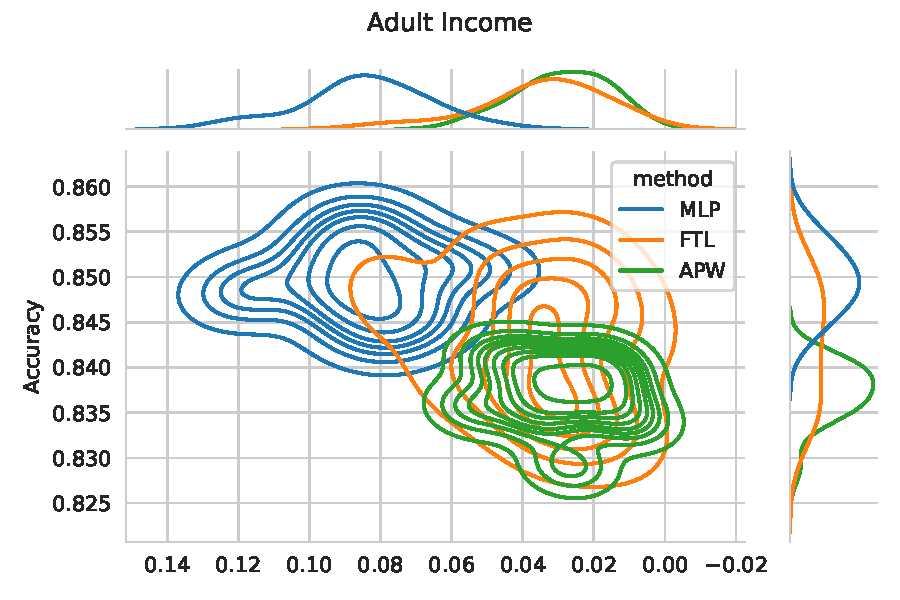
\includegraphics[width=1\linewidth]{images/pareto_acc_odds_adult.pdf}
\end{subfigure}
\begin{subfigure}{.45\linewidth}
    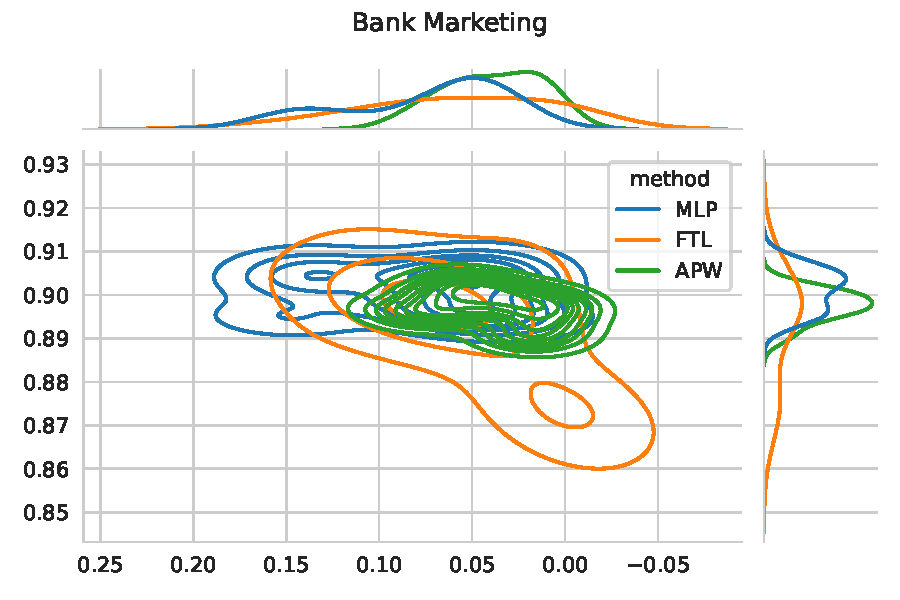
\includegraphics[width=1\linewidth]{images/pareto_acc_odds_bank.pdf}
\end{subfigure}

\begin{subfigure}{.45\linewidth}
    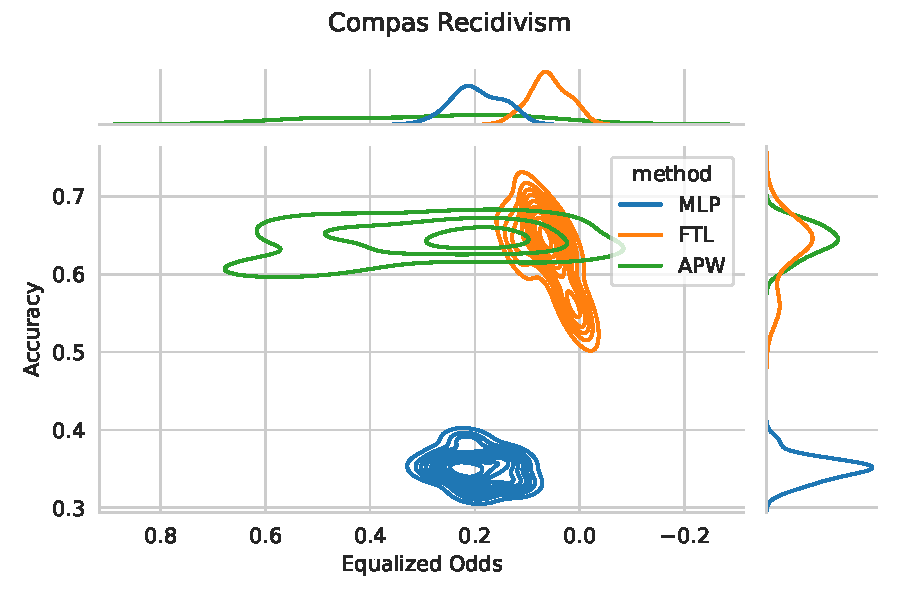
\includegraphics[width=1\linewidth]{images/pareto_acc_odds_compas.pdf}
\end{subfigure}
\begin{subfigure}{.45\linewidth}
    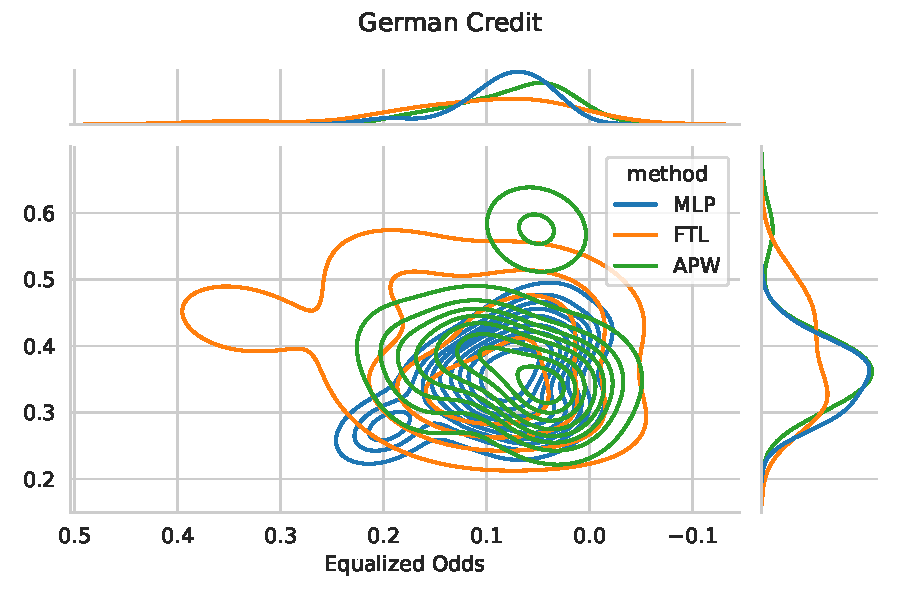
\includegraphics[width=1\linewidth]{images/pareto_mcc_odds_german.pdf}
\end{subfigure}
\end{figure}
